% Judul dokumen
\title{Buku Tugas Akhir ITS}
\author{Wicaksono, Agung}

% Pengaturan ukuran teks dan bentuk halaman dua sisi
\documentclass[10pt,twoside]{report}

% Pengaturan ukuran halaman dan margin
\usepackage[a5paper,top=25mm,left=25mm,right=20mm,bottom=25mm]{geometry}

% Pengaturan ukuran spasi
\usepackage[singlespacing]{setspace}

% Pengaturan format bahasa
\usepackage[indonesian]{babel}

% Pengaturan detail pada file PDF
\usepackage[pdfauthor={\@author},bookmarksnumbered,pdfborder={0 0 0}]{hyperref}

% Pengaturan jenis karakter
\usepackage[utf8]{inputenc}

% Pengaturan pewarnaan
\usepackage[table,xcdraw]{xcolor}

% Pengaturan kutipan artikel
\usepackage[numbers]{natbib}

\usepackage{amsmath}

% Package lainnya
\usepackage{changepage}
\usepackage{enumitem}
\usepackage{eso-pic}
\usepackage{etoolbox}
\usepackage{graphicx}
\usepackage{lipsum}
\usepackage{lmodern}
\usepackage{longtable}
\usepackage{tabularx}
\usepackage{wrapfig}
\usepackage[pageref]{backref}

% Definisi untuk "Hati ini sengaja dikosongkan"
\patchcmd{\cleardoublepage}{\hbox{}}{
  \thispagestyle{empty}
  \vspace*{\fill}
  \begin{center}\textit{[Halaman ini sengaja dikosongkan]}\end{center}
  \vfill}{}{}

% Untuk citation
\newcommand{\tab}[1]{\hspace{.2\textwidth}\rlap{#1}}
\renewcommand*{\backreflastsep}{, }
\renewcommand*{\backreftwosep}{, }
\renewcommand*{\backref}[1]{}
\renewcommand*{\backrefalt}[4]{
	\ifcase #1
	No citations.
	\or
	(Dikutip pada halaman #2).
	\else
	(Dikutip pada halaman #2).
	\fi
}


% Pengaturan penomoran halaman
\usepackage{fancyhdr}
\fancyhf{}
\renewcommand{\headrulewidth}{0pt}
\pagestyle{fancy}
\fancyfoot[CE,CO]{\thepage}
\patchcmd{\chapter}{plain}{fancy}{}{}
\patchcmd{\chapter}{empty}{plain}{}{}

% Pengaturan format judul bab
\usepackage{titlesec}
\titleformat{\chapter}[display]{\bfseries\Large}{BAB \centering\Roman{chapter}}{0ex}{\vspace{0ex}\centering}
\titleformat{\section}{\bfseries\large}{\MakeUppercase{\thesection}}{1ex}{\vspace{1ex}}
\titleformat{\subsection}{\bfseries\large}{\MakeUppercase{\thesubsection}}{1ex}{}
\titleformat{\subsubsection}{\bfseries\large}{\MakeUppercase{\thesubsubsection}}{1ex}{}
\titlespacing{\chapter}{0ex}{0ex}{4ex}
\titlespacing{\section}{0ex}{1ex}{0ex}
\titlespacing{\subsection}{0ex}{0.5ex}{0ex}
\titlespacing{\subsubsection}{0ex}{0.5ex}{0ex}


% Pengaturan format potongan kode
\usepackage{listings}
\definecolor{comment}{RGB}{0,128,0}
\definecolor{string}{RGB}{255,0,0}
\definecolor{keyword}{RGB}{0,0,255}
\lstdefinestyle{codestyle}{
  commentstyle=\color{comment},
  stringstyle=\color{string},
  keywordstyle=\color{keyword},
  basicstyle=\footnotesize\ttfamily,
  numbers=left,
  numberstyle=\tiny,
  numbersep=5pt,
  frame=lines,
  breaklines=true,
  prebreak=\raisebox{0ex}[0ex][0ex]{\ensuremath{\hookleftarrow}},
  showstringspaces=false,
  upquote=true,
  tabsize=2,
}
\lstset{style=codestyle}

% Isi keseluruhan dokumen
\begin{document}

  % Sampul luar
  \AddToShipoutPictureBG*{
  \AtPageLowerLeft{
    % Ubah nilai berikut jika posisi horizontal background tidak sesuai
    \hspace{-3.5mm}

    % Ubah nilai berikut jika posisi vertikal background tidak sesuai
    \raisebox{0mm}{
      
\includegraphics[width=\paperwidth,height=\paperheight]{sampul/gambar/sampul-luar.png}
    }
  }
}

% Menyembunyikan nomor halaman
\thispagestyle{empty}

% Pengaturan margin untuk menyesuaikan konten sampul
\newgeometry{
  top=95mm,
  left=25mm,
  right=20mm,
  bottom=25mm
}

\begin{flushleft}

  % Pemilihan font sans serif
  \sffamily

  % Pemilihan warna font putih
  \color{white}

  % Pemilihan font bold
  \fontseries{bx}
  \selectfont

  % Ubah penomoran buku berikut dengan yang ditentukan oleh departemen
TUGAS AKHIR - EC184801

\vspace{6ex}

% Ubah kalimat berikut dengan judul tugas akhir
\begin{large}
  DETEKSI PEJALAN KAKI PADA \textit{ZEBRACROSS} UNTUK PERINGATAN DINI PENGENDARA MOBIL MENGGUNAKAN \textit{MASK R-CNN}
\end{large}

\vspace{4ex}

% Ubah kalimat-kalimat berikut dengan nama dan NRP mahasiswa
Agung Wicaksono \\
NRP 0721 17 4000 0002

\vspace{2ex}

% Ubah kalimat-kalimat berikut dengan nama-nama dosen pembimbing
Dosen Pembimbing \\
Prof. Dr. Ir. Mauridhi Hery Purnomo, M.Eng.\\
Dr. Eko Mulyanto Yuniarno, S.T., M.T.

\vspace{6ex}

% Ubah kalimat-kalimat berikut dengan nama departemen dan fakultas
DEPARTEMEN TEKNIK KOMPUTER \\
Fakultas Teknologi ELEKTRO DAN INFORMATIKA CERDAS \\
Institut Teknologi Sepuluh Nopember

% Ubah kalimat berikut dengan tempat dan tahun pembuatan buku
Surabaya 2021


\end{flushleft}

\restoregeometry


  % Sampul dalam
  \AddToShipoutPictureBG*{
  \AtPageLowerLeft{
    % Ubah nilai berikut jika posisi horizontal background tidak sesuai
    \hspace{-3.5mm}

    % Ubah nilai berikut jika posisi vertikal background tidak sesuai
    \raisebox{0mm}{
      
\includegraphics[width=\paperwidth,height=\paperheight]{sampul/gambar/sampul-dalam.png}
    }
  }
}

% Menyembunyikan nomor halaman
\thispagestyle{empty}

% Pengaturan margin untuk menyesuaikan konten sampul
\newgeometry{
  top=95mm,
  left=25mm,
  right=20mm,
  bottom=25mm
}

\begin{flushleft}

  % Pemilihan font sans serif
  \sffamily

  % Pemilihan font bold
  \fontseries{bx}
  \selectfont

  % Ubah penomoran buku berikut dengan yang ditentukan oleh departemen
TUGAS AKHIR - EC184801

\vspace{6ex}

% Ubah kalimat berikut dengan judul tugas akhir
\begin{large}
  DETEKSI PEJALAN KAKI PADA \textit{ZEBRACROSS} UNTUK PERINGATAN DINI PENGENDARA MOBIL MENGGUNAKAN \textit{MASK R-CNN}
\end{large}

\vspace{4ex}

% Ubah kalimat-kalimat berikut dengan nama dan NRP mahasiswa
Agung Wicaksono \\
NRP 0721 17 4000 0002

\vspace{2ex}

% Ubah kalimat-kalimat berikut dengan nama-nama dosen pembimbing
Dosen Pembimbing \\
Prof. Dr. Ir. Mauridhi Hery Purnomo, M.Eng.\\
Dr. Eko Mulyanto Yuniarno, S.T., M.T.

\vspace{6ex}

% Ubah kalimat-kalimat berikut dengan nama departemen dan fakultas
DEPARTEMEN TEKNIK KOMPUTER \\
Fakultas Teknologi ELEKTRO DAN INFORMATIKA CERDAS \\
Institut Teknologi Sepuluh Nopember

% Ubah kalimat berikut dengan tempat dan tahun pembuatan buku
Surabaya 2021


\end{flushleft}

\restoregeometry

  \cleardoublepage

  % Pengaturan ukuran indentasi paragraf
  \setlength{\parindent}{2em}

  % Pengaturan ukuran spasi paragraf
  \setlength{\parskip}{1ex}

  % Pernyataan keaslian
  \begin{center}
  \large
  \textbf{PERNYATAAN KEASLIAN\\TUGAS AKHIR}
\end{center}

% Menyembunyikan nomor halaman
\thispagestyle{empty}

\vspace{2ex}

% Ubah paragraf-paragraf berikut sesuai dengan yang ingin diisi pada pernyataan keaslian

Dengan ini saya menyatakan bahwa isi sebagian maupun keseluruhan Tugas Akhir sada dengan judul \textbf{"Deteksi Pejalan Kaki pada \textit{Zebra Cross} untuk Peringatan Dini Pengendara Mobil menggunakan Mask R-CNN"} adalah benar-benar hasil karya intelektual mandiri, diselesaikan tanpa menggunakan bahan-bahan yang tidak diijinkan da bukan karya pihak lain yang saya akui sebagai karya sendiri.

Semua referensi yang dikutip maupun dirujuk telah ditulis secara lengkap pada daftar pustaka.

Apabila ternyata pernyataan ini tidak benar, saya bersedia menerima sanksi sesuai peraturan yang berlaku.

\vspace{4ex}

\begin{flushright}
  \begin{tabular}[b]{c}
    % Ubah kalimat berikut sesuai dengan tempat, bulan, dan tahun penulisan
    Surabaya, 14 Juni 2021\\
    \\
    \\
    \\
    \\
    % Ubah kalimat-kalimat berikut sesuai dengan nama dan NRP mahasiswa
    Agung Wicaksono\\
    0721 17 4000 0002
  \end{tabular}
\end{flushright}

  \cleardoublepage

  % Lembar pengesahan
  \begin{center}
	\large
  \textbf{LEMBAR PENGESAHAN}
\end{center}

% Menyembunyikan nomor halaman
\thispagestyle{empty}

\begin{center}
  % Ubah kalimat berikut dengan judul tugas akhir
  \textbf{DETEKSI PEJALAN KAKI PADA \textit{ZEBRACROSS} UNTUK PERINGATAN DINI PENGENDARA MOBIL MENGGUNAKAN \textit{MASK R-CNN}}
\end{center}

\begingroup
  % Pemilihan font ukuran small
  \small

  \begin{center}
    % Ubah kalimat berikut dengan pernyataan untuk lembar pengesahan
    Tugas Akhir ini disusun untuk memenuhi salah satu syarat memperoleh gelar Sarjana Teknik di Institut Teknologi Sepuluh Nopember Surabaya
  \end{center}

  \begin{center}
    % Ubah kalimat berikut dengan nama dan NRP mahasiswa
    Oleh: Agung Wicaksono (NRP. 0721 17 4000 0002)
  \end{center}

  \begin{center}
    % Ubah kalimat-kalimat berikut dengan tanggal ujian dan periode wisuda
    Tanggal Ujian :  Juli 2021\\
    Periode Wisuda : September 2021
  \end{center}

  \begin{center}
    Disetujui Oleh:
  \end{center}

  \begingroup
    % Menghilangkan padding
    \setlength{\tabcolsep}{0pt}

    \noindent
    \begin{tabularx}{\textwidth}{X c}
      % Ubah kalimat-kalimat berikut dengan nama dan NIP dosen pembimbing pertama
      Prof. Dr. Ir. Mauridhi Hery Purnomo, M.Eng.          & (Pembimbing I) \\
      NIP: 	19580916 198601 1 001       & ................................... \\
      &  \\
      &  \\
      % Ubah kalimat-kalimat berikut dengan nama dan NIP dosen pembimbing kedua
      Dr. Eko Mulyanto Yuniarno, S.T., M.T.     & (Pembimbing II) \\
      NIP: 19680601 199512 1 009        & ................................... \\
      &  \\
      &  \\
      % Ubah kalimat-kalimat berikut dengan nama dan NIP dosen penguji pertama
      Dosen Penguji Pertama.  & (Penguji I) \\
      NIP: 00000000 000000 0 000        & ................................... \\
      &  \\
      &  \\
      % Ubah kalimat-kalimat berikut dengan nama dan NIP dosen penguji kedua
      Dosen Penguji Kedua.  & (Penguji II) \\
      NIP: 00000000 000000 0 000        & ................................... \\
      &  \\
      &  \\
      % Ubah kalimat-kalimat berikut dengan nama dan NIP dosen penguji ketiga
      Dosen Penguji Ketiga.             & (Penguji III) \\
      NIP: 00000000 000000 0 000        & ................................... \\
    \end{tabularx}
  \endgroup

  \vspace{1ex}

  \begin{center}
    % Ubah kalimat berikut dengan jabatan kepala departemen
    Mengetahui, \\
    Kepala Departemen Teknik Komputer FTEIC - ITS \\

    \vspace{7ex}

    % Ubah kalimat-kalimat berikut dengan nama dan NIP kepala departemen
    \underline{Dr. Supeno Mardi Susiki Nugroho, ST., MT.} \\
    NIP. 19700313 199512 1 001
  \end{center}
\endgroup

  \cleardoublepage

  % Nomor halaman pembuka dimulai dari sini
  \pagenumbering{roman}

  % Abstrak Bahasa Indonesia
  \begin{center}
  \large\textbf{ABSTRAK}
\end{center}

\addcontentsline{toc}{chapter}{ABSTRAK}

\vspace{2ex}

\begingroup
  % Menghilangkan padding
  \setlength{\tabcolsep}{0pt}

  \noindent
  \begin{tabularx}{\textwidth}{l >{\centering}m{2em} X}
    % Ubah kalimat berikut dengan nama mahasiswa
    Nama Mahasiswa    &:& Elon Reeve Musk \\

    % Ubah kalimat berikut dengan judul tugas akhir
    Judul Tugas Akhir &:&	Kalkulasi Energi pada Roket Luar Angkasa Berbasis \emph{Anti-Gravitasi} \\

    % Ubah kalimat-kalimat berikut dengan nama-nama dosen pembimbing
    Pembimbing        &:& 1. Nikola Tesla, S.T., M.T. \\
                      & & 2. Wernher von Braun, S.T., M.T. \\
  \end{tabularx}
\endgroup

% Ubah paragraf berikut dengan abstrak dari tugas akhir
Pada penelitian ini kami mengajukan \lipsum[1]

% Ubah kata-kata berikut dengan kata kunci dari tugas akhir
Kata Kunci: Roket, \emph{Anti-gravitasi}, Energi, Angkasa.

  \cleardoublepage

  % Abstrak Bahasa Inggris
  \begin{center}
  \large\textbf{ABSTRACT}
\end{center}

\addcontentsline{toc}{chapter}{ABSTRACT}

\vspace{2ex}

\begingroup
  % Menghilangkan padding
  \setlength{\tabcolsep}{0pt}

  \noindent
  \begin{tabularx}{\textwidth}{l >{\centering}m{3em} X}
    % Ubah kalimat berikut dengan nama mahasiswa
    \emph{Name}     &:& Agung Wicaksono \\

    % Ubah kalimat berikut dengan judul tugas akhir dalam Bahasa Inggris
    \emph{Title}    &:& \emph{Pedestrian Detection on \textit{Zebra Cross} for Car Driver Early Warning using \textit{Mask R-CNN}} \\

    % Ubah kalimat-kalimat berikut dengan nama-nama dosen pembimbing
    \emph{Advisors}  &:& 1. Prof. Dr. Ir. Mauridhi Hery Purnomo, M.Eng. \\
    				 & & 2. Dr. Eko Mulyanto Yuniarno, S.T., M.T. \\
  \end{tabularx}
\endgroup

% Ubah paragraf berikut dengan abstrak dari tugas akhir dalam Bahasa Inggris
\emph{Today, safety features on four-wheeled vehicles or cars have developed very rapidly. This is evidenced by the number of car manufacturers that apply seat belt technology, air bags, adaptive cruise control, electronic stability control, autonomous emergency braking, blind spot monitoring and so on. However, the features mentioned above are still considered less friendly for pedestrians. It is proven that according to data from the WHO, there are 270,000 pedestrians who die every year or about 22\% of all victims die due to road accidents. Starting from these problems, the author will conduct research on the detection of pedestrians at zebra cross for early warning car drivers as a research topic. In this final project, there are 3 objects to be detected, namely pedestrians, zebra cross and motorcyclists using the Mask R-CNN method. The best results obtained are the use of \textit{ResNet-101} for \textit{backbone Mask R-CNN} with a score of \textit{mAP} of 76,605\%, mAR of 85.375\% and \textit{F1-Score} of 80.302\% .}

% Ubah kata-kata berikut dengan kata kunci dari tugas akhir dalam Bahasa Inggris
\emph{Keywords}: \emph{Pedestrian, Zebra Cross, Mask R-CNN, Image Processing}

  \cleardoublepage

  % Kata pengantar
  \begin{center}
  \Large
  \textbf{KATA PENGANTAR}
\end{center}

% Ubah paragraf-paragraf berikut dengan isi dari kata pengantar

Puji dan syukur kehadirat Tuhan Yang Maha Esa atas segala karunia-Nya, penulis  dapat menyelesaikan penelitian ini dengan judul \textbf{Deteksi Pejalan Kaki pada \textit{Zebracross} untuk Peringatan Dini Pengendara Mobil menggunakan \textit{Mask R-CNN}.}

Penelitian ini disusun dalam rangka pemenuhan bidang riset di Departemen Teknik Komputer ITS, sera digunakan sebagai persyaratan menyelesaikan pendidikan Sarjana. Penelitian ini dapat diselesaikan tidak lepas dari bantuan berbagai pihak. Oleh karena itu, penulis mengucapkan terimakasih kepada:

\begin{enumerate}[nolistsep]
  \item Keluarga, Ibu, Bapak dan Saudara tercinta yang telah memberikan dorongan baik secara spiritual dan material dalam penyelesaian buku penelitian ini.
  \item Bapak Dr. Supeno Mardi Susiki Nugroho, ST., MT. selaku Kepala Departemen Teknik Komputer, Fakultas Teknologi Elektro dan Informatika Cerdas, Institut Teknologi Sepuluh Nopember. 
  \item Bapak Prof. Dr. Ir. Mauridhi Hery Purnomo, M.Eng. selaku dosen pembimbing I dan Bapak Dr. Eko Mulyanto Yuniarno, S.T., M.T. selaku dosen pembimbing II yang selalu memberikan arahan selama mengerjakan penelitian tugas akhir ini.
  \item Bapak-ibu dosen pengajar Departemen Teknik Komputer, atas pengajaran dam bimbingan yang diberikan kepada penulis.
  \item Seluruh teman-teman dari angkatan e57, Teknik Komputer, Laboratorium B401 dan B201 Teknik Komputer ITS serta Saturasi ITS.
\end{enumerate}

Kesempurnaan hanya milik Allah SWT, untuk itu penulis memohon segenap kritik dan saran yang membangun. Semoga penelitian ini dapat memberikan manfaat bagi kita semua. Amin.


\begin{flushright}
  \begin{tabular}[b]{c}
    % Ubah kalimat berikut dengan tempat, bulan, dan tahun penulisan
    Surabaya, 9 Juli 2021\\
    \\
    \\
    \\
    \\
    % Ubah kalimat berikut dengan nama mahasiswa
    Agung Wicaksono
  \end{tabular}
\end{flushright}

  \cleardoublepage

  % Daftar isi
  \renewcommand*\contentsname{DAFTAR ISI}
  \addcontentsline{toc}{chapter}{\contentsname}
  \tableofcontents
  \cleardoublepage

  % Daftar gambar
  \renewcommand*\listfigurename{DAFTAR GAMBAR}
  \addcontentsline{toc}{chapter}{\listfigurename}
  \listoffigures
  \cleardoublepage

  % Daftar tabel
  \renewcommand*\listtablename{DAFTAR TABEL}
  \addcontentsline{toc}{chapter}{\listtablename}
  \listoftables
  \cleardoublepage

  % Nomor halaman isi dimulai dari sini
  \pagenumbering{arabic}

  % Bab 1 pendahuluan
  \chapter{PENDAHULUAN}
\label{chap:pendahuluan}

% Ubah bagian-bagian berikut dengan isi dari pendahuluan

Penelitian ini di latar belakangi oleh berbagai kondisi yang menjadi acuan. Selain itu juga terdapat beberapa permasalahan yang akan dijawab sebagai luaran dari penelitian.

\section{Latar Belakang}
\label{sec:latarbelakang}

Mobil merupakan salah satu jenis kendaraan bermotor yang banyak terdapat di Indonesia. Pada tahun 2018 Badan Pusat Statistik mencatat terdapat 16.440.987 mobil penumpang yang berada di Indonesia. Dengan bertambahnya jumlah mobil di Indonesia dari tahun ke tahun, meningkatkan juga jumlah kecelakaan mobil. Fitur keselamatan dan keamanan pada mobil sangat penting bagi para pengendara dan penumpang, sehingga para produsen mobil berusaha meningkatkan teknologi keselamatan dan keamanan pada mobil buatannya. Sebagai contoh beberapa fitur keselamatan dan keamanan yang
terdapat pada mobil antara lain, adaptive cruise control, hill strat assist, blind spot monitoring, electronic stability control dan lain sebagainya.

Menurut data dari WHO, terdapat 270.000 pejalan kaki meninggal dunia setiap tahun atau sekitar 22\% dari seluruh korban meniggal akibat kecelakan di jalan. Melihat kegiatan para pejalan kaki yang jarang berada di badan jalan, angka tersebut tentu cukup tinggi. Para pejalan kaki hanya menggunakan badan jalan ketika hendak menyebrang jalan lewat zebracross. Kelalaian dari pejalan kaki maupun pengendara mobil merupakan faktor utama mengapa angka kematian pejalan kaki cukup tinggi. Salah satu contoh kelalaian pejalan kaki adalah pada saat menyebrang jalan tidak memperhatikan kendaraan yang akan lewat dan atau melihat rambu serta lampu lalu lintas. Di sisi pengendara mobil, kelelahan,
kurangnya fokus saat berkendara dan tidak memperhatikan rambu maupun marka dapat berakibat fatal
baik kepada pejalan kaki dan pengendara lain.

Teknologi artificial intelligent sudah banyak disematkan pada mobil pada masa kini, dibuktikan
dengan adanya teknologi adaptive cruise control, hill start assist dan lain sebagainya. Artificial intelligent khususnya deep learning tentu dapat digunakan untuk deteksi pejalan kaki di zebracross guna mengurangi jumlah korban akibat kecelakaan. Deteksi pejalan kaki dapat digabungkan dengan buzzer dan atau LED sebagai komponen output untuk mengingatkan kepada pengendara bahwa ada pejalan kaki yang sedang menyebrangi jalan serta mengembalikan fokus untuk berkendara.

\section{Permasalahan}
\label{sec:permasalahan}

Cukup tingginya angka kematian pejalan kaki akibat kecelakaan lalu lintas dan belum adanya deteksi pejalan kaki di zebracross untuk peringatan dini kepada pengendara mobil. Oleh karena itu, diperlukan sebuah sistem yang mampu mendeteksi adanya pejalan kaki yang berada disekitar jalan raya untuk selanjutnya dapat digunakan sebagai peringatan kepada pengendara mobil.

\section{Tujuan}
\label{sec:Tujuan}

Berdasarkan rumusan permasalahan di atas, tujuan dari penelitian ini adalah untuk mendeteksi adanya pejalan kaki di zebracross untuk peringatan dini kepada pengendara mobil guna mengurangi angka kematian pejalan kaki akibat kecelakaan lalu lintas

\section{Batasan Masalah}
\label{sec:batasanmasalah}

Batasan-batasan dari \lipsum[1][1-3] adalah:

\begin{enumerate}[nolistsep]

  \item Mempermudah \lipsum[2][1-3]

  \item \lipsum[3][1-5]

  \item \lipsum[4][1-5]

\end{enumerate}

\section{Sistematika Penulisan}
\label{sec:sistematikapenulisan}

Laporan penelitian tugas akhir ini tersusun dalam sistematika dan terstruktur sehingga mudah dipahami dan dipelajari oleh pembaca maupun seseorang yang ingin melanjutkan penelitian ini. Alur sistematika penulisan laporan penelitian ini yaitu :

\begin{enumerate}[nolistsep]

  \item \textbf{BAB I Pendahuluan}

  Bab ini berisi uraian tentang latar belakang permasalahan, penegasan dan alasan pemilihan judul, sistematika laporan, tujuan dan metodologi penelitian.

  \vspace{2ex}

  \item \textbf{BAB II Tinjauan Pustaka}

  Pada bab ini berisi tentang uraian secara sistematis teori-teori yang berhubungan dengan permasalahan yang dibahas pada penelitian ini. Teori-teori ini digunakan sebagai dasar dalam penelitian, yaitu informasi terkait 
  dan teori-teori penunjang lainya.

  \vspace{2ex}

  \item \textbf{BAB III Desain dan Implementasi Sistem}

  Bab ini berisi \lipsum[4][1-5]

  \vspace{2ex}

  \item \textbf{BAB IV Pengujian dan Analisa}

  Bab ini berisi \lipsum[5][1-5]

  \vspace{2ex}

  \item \textbf{BAB V Penutup}

  Bab ini berisi \lipsum[6][1-5]

\end{enumerate}

  \cleardoublepage

  % Bab 2 tinjauan pustaka
  \chapter{TINJAUAN PUSTAKA}
\label{chap:tinjauanpustaka}

% Ubah bagian-bagian berikut dengan isi dari tinjauan pustaka

Demi mendukung penelitian ini, dibutuhkan beberapa teori penunjang sebagai bahan acuan dan refrensi. Dengan demikian penelitian ini menjadi lebih terarah.

\section{Dasar Teori}
\label{sec:dasarteori}

\subsection{\textit{Artificial Intelligence}}
\label{subsec:artificial-itelligence}

\textit{Artificial Intelligence} mengacu pada simulasi kecerdasan manusia dalam mesin yang diprogram untuk berpikir seperti manusia dan meniru tindakan mereka.\citep{artificialintellingece} Istilah ini juga dapat diterapkan pada mesin apa pun yang menunjukkan ciri-ciri yang terkait dengan pikiran manusia seperti pembelajaran dan pemecahan masalah.

Karakteristik ideal dari \textit{artificial intellingence} adalah kemampuannya untuk merasionalisasi dan mengambil tindakan yang memiliki peluang terbaik untuk mencapai tujuan tertentu. Bagian dari \textit{artificial intellingece} adalah \textit{machine learning}, yang mengacu pada konsep bahwa program komputer dapat secara otomatis belajar dari dan beradaptasi dengan data baru tanpa dibantu oleh manusia. Teknik\textit{deep learning} memungkinkan pembelajaran otomatis ini melalui penyerapan sejumlah besar data tidak terstruktur seperti teks, gambar, atau video.

\subsection{\textit{Machine Learning}}
\label{subsec:machine-learning}

\textit{Machine Learning} adalah studi tentang algoritma komputer yang memberikan sistem kemampuan untuk belajar secara otomatis dan dapat meningkatkan kemampuan dari pengalaman yang sudah didapatkan \citep{machinelearning1}. Hal ini umumnya dilihat sebagai sub-bidang kecerdasan buatan. Algoritma pembelajaran mesin memungkinkan sistem membuat keputusan secara mandiri tanpa dukungan eksternal. Keputusan semacam itu dibuat dengan menemukan pola dasar yang berharga dalam data yang kompleks. Berdasarkan pendekatan pembelajaran, jenis data \textit{input} dan \textit{output}, dan jenis masalah yang dipecahkan, ada beberapa kategori utama dari algoritma \textit{machine learning} \textit{supervised, unsupervised} dan \textit{reinforcement learning}. Ada beberapa pendekatan hibrida dan metode umum lainnya yang menawarkan ekstrapolasi alami dari bentuk masalah pembelajaran mesin. Berikut merupakan penjelasan dari beberapa kategori utama dari algoritma \textit{machine learning}:

\begin{enumerate}
	\item \textit{Supervised Learning} diterapkan ketika data dalam bentuk variabel input dan nilai target output. Algoritma akan mempelajari fungsi pemetaan dari \textit{input} ke \textit{output}. Ketersediaan sampel data berlabel dengan skala besar mempunyai nilai yang tinggi dikarenakan masih terdapat kelangkaan \textit{dataset}. Pendekatan ini secara luas dapat dibagi menjadi dua kategori utama yaitu \textit{classification} dan \textit{regression}. Gambar \ref{fig:supervised} menampilkan visualisasi dari \textit{classification} dan \textit{regression} pada \textit{Supervised Learning}
	
	\begin{figure}[ht]
		\centering
		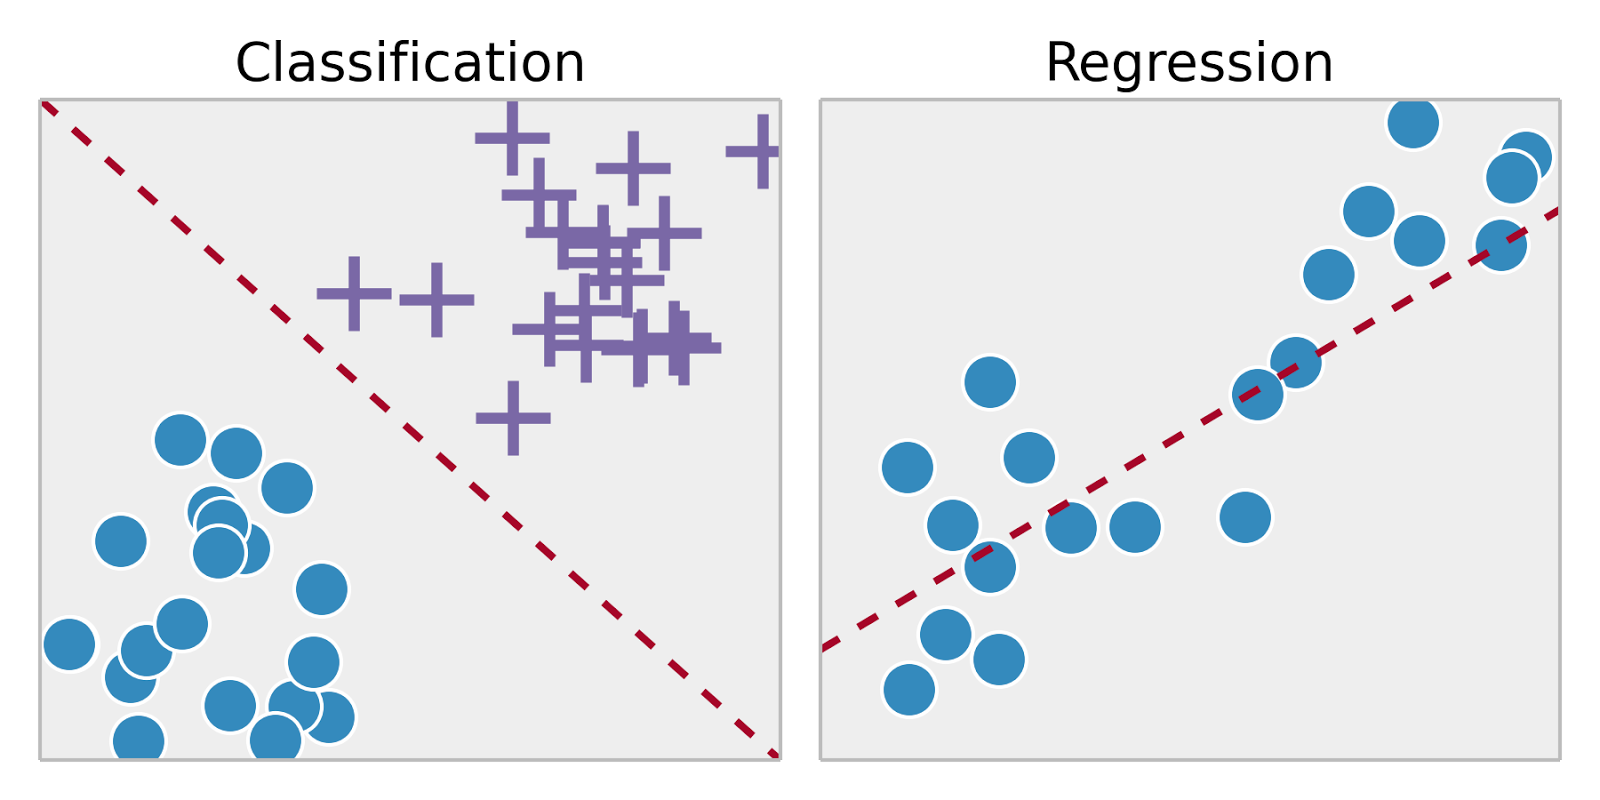
\includegraphics[scale=0.1]{gambar/supervised.png}
		\caption{Gambaran \textit{Supervised Learning}\citep{supervised}}
		\label{fig:supervised}
	\end{figure}  
	
	\item \textit{Unsupervised Learning} diterapkan ketika data hanya tersedia dalam bentuk \textit{input} dan tidak ada variabel \textit{output} yang sesuai. Algoritma semacam itu memodelkan pola yang mendasari data untuk mempelajari lebih lanjut tentang karakteristiknya. Salah satu jenis utama dari algoritma \textit{unsupervised} adalah pengelompokan. Dalam teknik ini, kelompok yang melekat dalam data ditemukan dan kemudian digunakan untuk memprediksi \textit{output} untuk \textit{input} yang tidak terlihat. Contoh dari teknik ini adalah untuk memprediksi perilaku pembelian pada pelanggan. Gambar \ref{fig:unsupervised} merupakan visualisasi dari algoritma \textit{unsupervised learning}.
	
	\begin{figure}[ht]
		\centering
		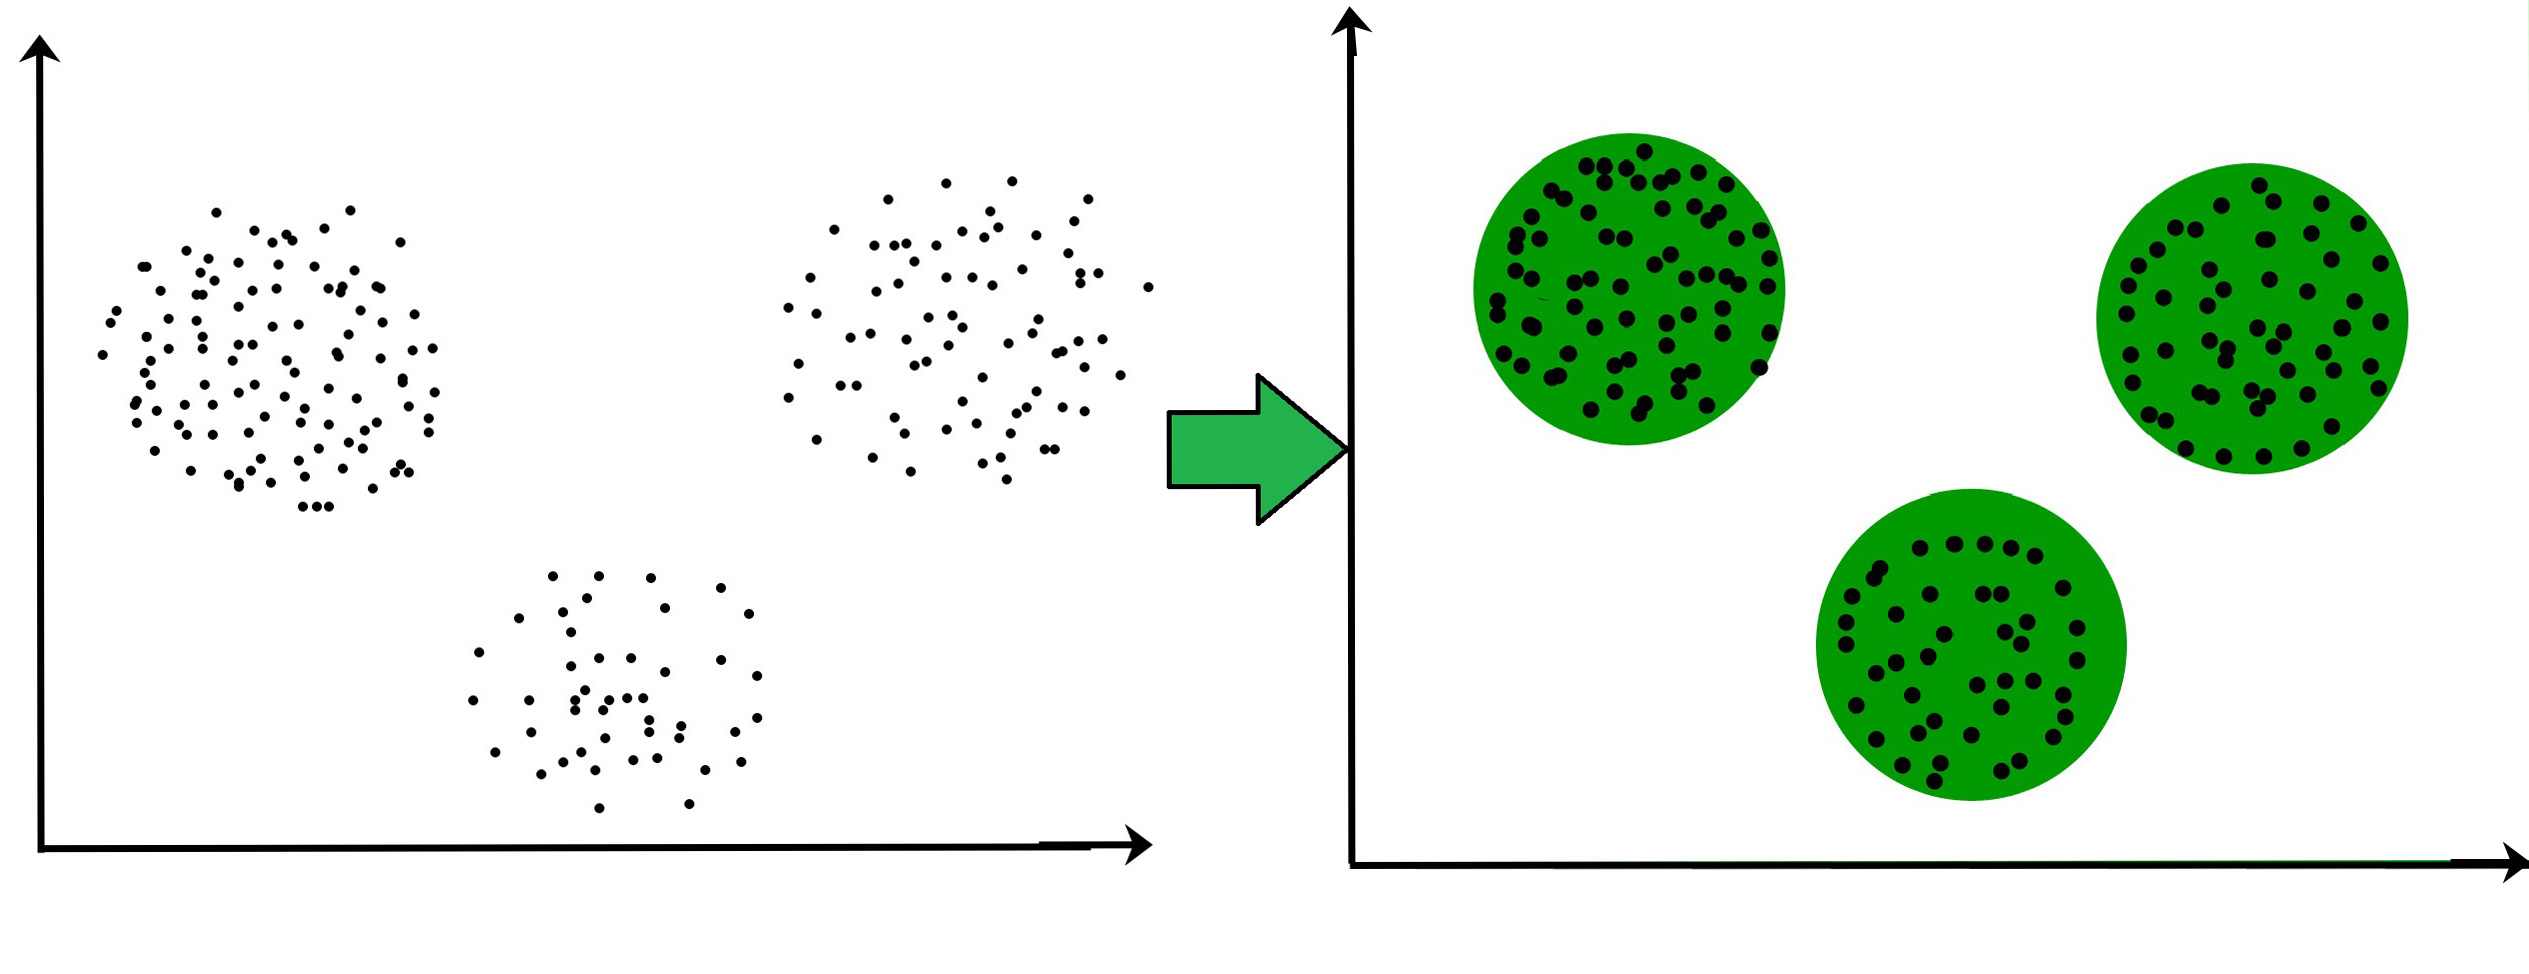
\includegraphics[scale=0.2]{gambar/unsupervised.jpg}
		\caption{Gambaran \textit{Unsupervised Learning}\citep{unsupervised}}
		\label{fig:unsupervised}
	\end{figure}
	
	
	\item \textit{Reinforcement learning} diterapkan ketika tugas yang ada
	adalah membuat urutan keputusan menuju \textit{reward} akhir. Selama proses \textit{learning}, \textit{artificial agent} mendapat \textit{reward} atau \textit{penalties} atas tindakan yang dilakukannya. Tujuannya adalah untuk memaksimalkan total \textit{reward} yang didapatkan. Gambar \ref{fig:reinforcement} merupakan visualisasi dari algoritma \textit{reinforcement learning}.
	
	\begin{figure}[ht]
		\centering
		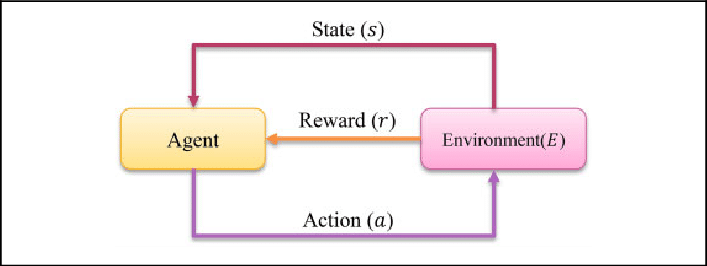
\includegraphics[scale=0.3]{gambar/reinforcement.png}
		\caption{Gambaran \textit{Reinforcement Learning}\citep{reinforcement}}
		\label{fig:reinforcement}
	\end{figure}
\end{enumerate}

\subsection{\textit{Deep Learning}}
\label{subsec:deeplearning}

\textit{Deep Learning} adalah kelas \textit{machine learning} yang berkinerja jauh lebih baik pada data tidak terstruktur\citep{dl}. Teknik \textit{deep learning} mengungguli teknik \textit{machine learning} saat ini. Ini memungkinkan model komputasi untuk mempelajari fitur secara progresif dari data di berbagai level. Popularitas \textit{deep learning} diperkuat karena jumlah data yang tersedia meningkat serta kemajuan perangkat keras yang menyediakan komputer yang kuat.

Arsitektur \textit{deep learning} berkinerja lebih baik daripada jaringan saraf tiruan  sederhana, meskipun waktu \textit{learning} dari struktur \textit{deep learning} lebih tinggi dari jaringan saraf tiruan. Namun, waktu \textit{learning} dapat dikurangi dengan menggunakan metode seperti \textit{transfer learning} atau komputasi menggunakan GPU. Salah satu faktor yang menentukan keberhasilan jaringan saraf terletak pada desain arsitektur jaringan yang cermat.

\subsection{\textit{Convolutional Neural Network}}
\label{subsec:cnn}

\textit{Convolutional Neural Networl} (CNN) adalah jenis khusus dari \textit{multilayer neural network} atau arsitektur \textit{deep learning} yang terinspirasi oleh sistem visual makhluk hidup \citep{cnn}. CNN sangat cocok untuk berbagai bidang visi komputer dan \textit{natural language processing}. \textit{Convolutional Neural Network} (CNN), juga disebut \textit{ConvNet}, adalah jenis \textit{Artificial Neural Network} (ANN), yang memiliki arsitektur \textit{feed-forward} yang dalam dan memiliki kemampuan generalisasi yang luar biasa dibandingkan dengan jaringan lain dengan lapisan FC (\textit{Fully Connected}), ia dapat mempelajari fitur objek yang sangat abstrak terutama data spasial dan dapat mengidentifikasinya dengan lebih efisien. Model CNN yang dalam terdiri dari satu set lapisan pemrosesan yang dapat mempelajari berbagai fitur data \textit{input} (misalnya gambar) dengan beberapa tingkat abstraksi seperti yang ditampilkan pada Gambar \ref{fig:concept-cnn}. Lapisan inisiator mempelajari dan mengekstrak fitur tingkat tinggi (dengan abstraksi yang lebih rendah), dan lapisan yang lebih dalam mempelajari dan mengekstrak fitur tingkat rendah (dengan abstraksi yang lebih tinggi).

\begin{figure}[ht]
	\centering
	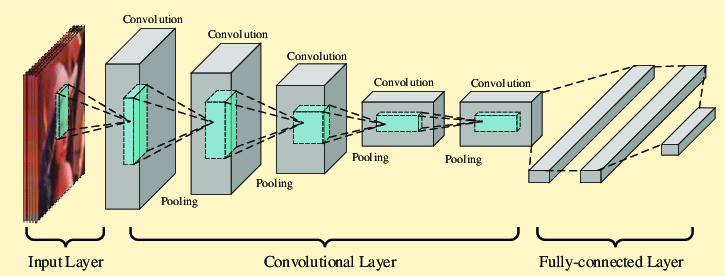
\includegraphics[scale=0.3]{gambar/concept-cnn.png}
	\caption{Gambaran Konsep Arsitektur CNN \citep{concept-cnn}}
	\label{fig:concept-cnn}
\end{figure}

\textit{Convolutional Neural Network} memiliki beberapa keunggulan dibanding dengan jaringan saraf tiruan lainnya dalam konteks visi komputer, antara lain :

\begin{enumerate}
	\item Salah satu alasan utama untuk mempertimbangkan CNN dalam kasus tersebut adalah fitur pembagian bobot dari CNN, yang mengurangi jumlah parameter yang dapat dilatih dalam jaringan, yang membantu model untuk menghindari \textit{overfitting} dan juga untuk meningkatkan generalisasi.
	\item Pada CNN, lapisan klasifikasi dan lapisan ekstraksi fitur melakukan proses \textit{learning} secara bersama-sama, yang membuat output model lebih terorganisir dan membuat output lebih bergantung pada fitur yang diekstraksi.
	\item Implementasi pada jaringan dengan ukuran yang besar akan lebih sulit dilakukan dengan menggunakan jenis jaringan saraf lain daripada menggunakan \textit{Convolutional Neural Network}
\end{enumerate}

\subsection{\textit{Convolutional Layer}}
\label{subsec:convolutional-layer}

\textit{Convolutional layer} adalah komponen terpenting dari arsitektur CNN mana pun. Ini berisi satu set kernel convolutional (juga disebut filter), yang dililitkan dengan gambar input (metrik N-dimensi) untuk menghasilkan peta fitur keluaran. Kernel dapat digambarkan sebagai kisi nilai atau angka diskrit, di mana setiap nilai dikenal sebagai bobot kernel. Selama awal proses pelatihan model CNN, semua bobot kernel ditetapkan dengan angka acak (pendekatan yang berbeda juga tersedia untuk inisialisasi bobot). Kemudian, dengan setiap periode \textit{learning}, bobot disetel dan kernel belajar mengekstrak fitur yang memberikan informasi mengenai data.

Pada \textit{Convolutional layer} terdapat istilah kernel yang mempunyai peran penting dalam proses yang dinamakan \textit{convolutional operation}. Kernel dapat digambarkan sebagai kisi nilai atau angka diskrit, di mana setiap nilai dikenal sebagai bobot kernel ini. Selama awal proses pelatihan model CNN, semua bobot kernel ditetapkan dengan angka acak (pendekatan yang berbeda juga tersedia di sana untuk menginisialisasi bobot). Kemudian, dengan setiap periode pelatihan, bobot disetel dan kernel belajar mengekstrak fitur yang berarti.

Sebelum kita mempelajari lebih jauh, mari kita pahami dulu format \textit{input} CNN. Berbeda dengan \textit{neural network} klasik lainnya dimana \textit{input}-nya dalam format vektor, di CNN \textit{input}-nya adalah gambar multi \textit{channel}. Misalnya untuk gambar RGB seperti pada Gambar \ref{fig:rgb-gray-image} mempunyai 3 \textit{channel} dan untuk gambar \textit{grayscale} hanya mempunyai satu \textit{channel}.

\begin{figure}[ht]
	\centering
	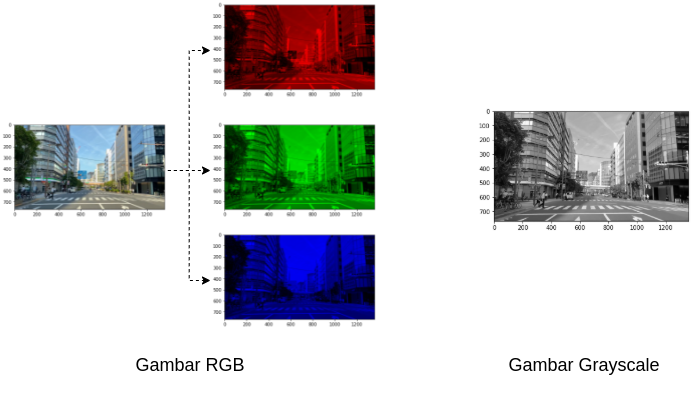
\includegraphics[scale=0.3]{gambar/rgb-gray-image.png}
	\caption{Contoh Gambar RGB dan Grayscale}
	\label{fig:rgb-gray-image}
\end{figure}

Sekarang, dalam operasi konvolusi, sebagai contoh diambil kernel 2 $\times$ 2 lalu diimplementasikan ke semua gambar 4 $\times$ 4 secara horizontal maupun vertikal dan sepanjang proses berlangsung dilakukan \textit{dot product} antara kernel dan gambar \textit{input} dengan mengalikan nilai yang sesuai dari keduanya dan dijumlahkan semua nilai untuk menghasilkan satu nilai skalar di \textit{feature map output}.Proses ini berlanjut hingga kernel tidak dapat lagi digeser lebih jauh. Untuk memahaminya secara lebih jelas, mari kita lakukan beberapa perhitungan awal yang dilakukan pada setiap langkah secara grafis seperti yang ditunjukkan pada Gambar \ref{fig:conv-step}, di mana setiap nilai kernel 2 $\times$ 2 (ditunjukkan dengan warna merah) berada dikalikan dengan wilayah berukuran sama (ditunjukkan dengan warna jingga) dalam gambar input 4 $\times$ 4 dan nilai yang dihasilkan dijumlahkan untuk mendapatkan entri yang sesuai (ditunjukkan dengan warna biru) di \textit{feature map output} pada setiap langkah konvolusi.

\begin{figure}[h!]
	\centering
	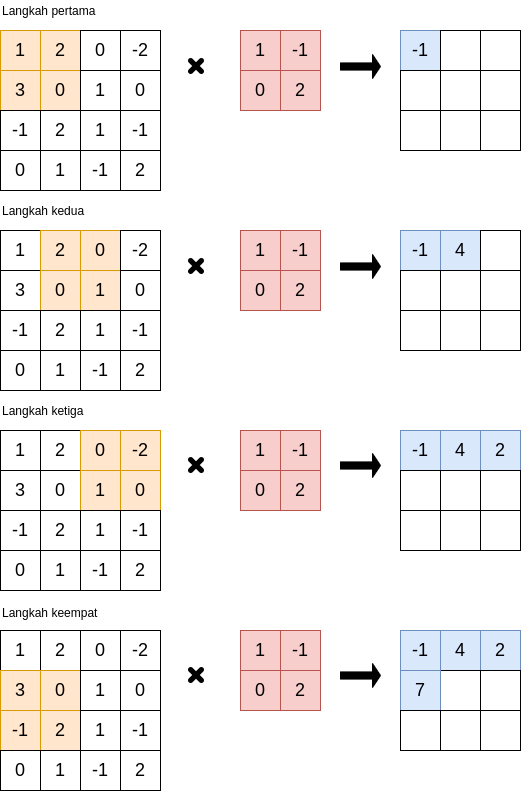
\includegraphics[scale=0.23]{gambar/langkah-konvolusi.png}
	\caption{Gambaran Operasi Konvolusi pada \textit{Convolution Layer}}
	\label{fig:conv-step}
\end{figure}

Dalam contoh di atas, diterapkan operasi konvolusi tanpa padding ke gambar masukan dan dengan \textit{stride} (yaitu ukuran langkah yang diambil sepanjang posisi horizontal atau vertikal ) sama dengan 1 ke kernel. Tapi bisa digunakan nilai \textit{stride} lain (bukan 1) dalam operasi konvolusi. Hal yang terlihat adalah jika kita meningkatkan langkah operasi konvolusi, itu menghasilkan \textit{feature map} berdimensi lebih rendah. \textit{Padding} penting untuk memberikan informasi ukuran batas dari input gambar jika tidak, tanpa menggunakan \textit{padding} apa pun, fitur sisi tepi akan terhapus terlalu cepat. \textit{Padding} juga digunakan untuk meningkatkan ukuran gambar \textit{input}, akibatnya ukuran \textit{feature map} \textit{output} juga meningkat. Gambar \ref{fig:conv-step-padd} memberikan contoh dengan menunjukkan operasi konvolusi dengan \textit{Zero-padding} dan 3 \textit{stride}. Rumus untuk mencari ukuran \textit{feature map} keluaran setelah operasi konvolusi adalah sebagai berikut:

\begin{equation}
	h'= \left[ \frac{h-f+p}{s} +1 \right]  
\end{equation}

\begin{equation}
	w'= \left[ \frac{w-f+p}{s} +1 \right]
\end{equation}

Dimana $h'$ menunjukkan tinggi dari \textit{feature map output}, $w'$ menunjukkan lebar dari \textit{feature map output}, $h$ menunjukkan tinggi dari gambar \textit{input}, $w$ menunjukkan lebar dari gambar \textit{input}, $f$ adalah ukuran filter, $p$ menunjukkan \textit{padding} dari operasi konvolusi dan $s$ menunjukkan \textit{stride} operasi konvolusi.

\begin{figure}[h!]
	\centering
	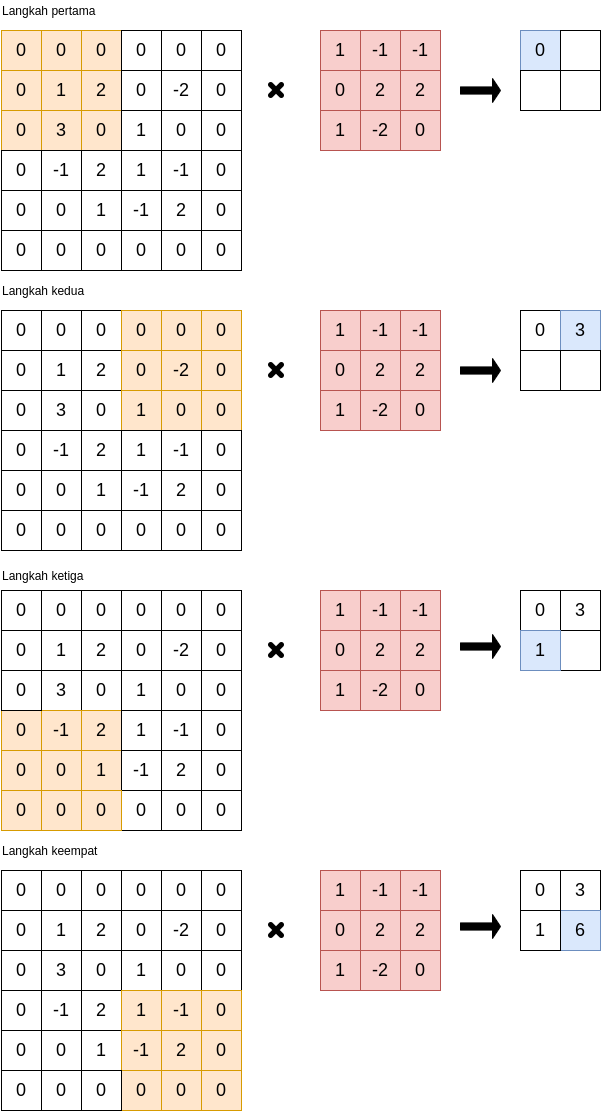
\includegraphics[scale=0.25]{gambar/conv-step-padd.png}
	\caption{Gambaran Operasi Konvolusi pada \textit{Convolution Layer} menggunakan \textit{Zero Padding}}
	\label{fig:conv-step-padd}
\end{figure}

Keuntungan utama dari lapisan konvolusi adalah:
\begin{enumerate}
	\item \textbf{\textit{Sparse Connectivity}}: Dalam jaringan saraf yang terhubung penuh, setiap \textit{neuron} dari satu lapisan terhubung dengan setiap \textit{neuron} dari lapisan berikutnya tetapi di CNN sejumlah kecil bobot terdapat di antara dua lapisan. Akibatnya, jumlah koneksi atau bobot yang kita butuhkan kecil, dan jumlah memori untuk menyimpan bobot itu juga kecil, sehingga hemat dalam penggunaan memori. Selain itu, operasi dot(.) secara komputasi lebih ringan daripada perkalian matriks.
	\item \textbf{\textit{Weight Sharing}}: Di CNN, tidak ada bobot khusus yang ada di antara dua neuron dari lapisan yang berdekatan melainkan semua bobot bekerja dengan setiap piksel dari matriks \textit{input}.Selain mempelajari bobot baru untuk setiap neuron, kita dapat mempelajari satu set bobot untuk semua input dan hal ini secara drastis dapat mengurangi waktu pelatihan.
\end{enumerate}

\subsection{\textit{Pooling Layer}}
\label{subsec:pooling-layer}

\textit{Pooling layer} digunakan untuk membuat sub-sampel \textit{feature map} (dihasilkan setelah operasi konvolusi), yaitu mengambil \textit{feature map} berukuran lebih besar dan mengecilkannya menjadi \textit{feature map} berukuran lebih kecil. Saat menyusutkan \textit{feature map}, \textit{pooling layer} tetap mempertahankan fitur (atau informasi) yang paling dominan di setiap langkah \textit{pools}. Operasi \textit{pooling} dilakukan dengan menentukan ukuran \textit{pooled region} dan langkah operasi, mirip dengan operasi konvolusi. Ada berbagai jenis teknik \textit{pooling} yang digunakan dalam berbagai \textit{pooling layer} seperti \textit{max pooling, min pooling, average pooling, gated pooling, tree pooling}, dan lain-lain. \textit{Max Pooling} adalah teknik pooling yang paling populer dan banyak digunakan.

Kelemahan utama dari \textit{pooling layer} adalah terkadang menurunkan kinerja CNN secara keseluruhan. Alasan di balik ini adalah bahwa lapisan penyatuan membantu CNN untuk menemukan apakah fitur tertentu ada dalam gambar masukan yang diberikan atau tidak tanpa memperhatikan posisi yang tepat dari fitur tersebut.

Gambar \ref{fig:max-pooling} mengilustrasikan contoh yang menunjukkan beberapa langkah awal serta keluaran akhir dari operasi \textit{max-pooling}, di mana ukuran area \textit{pooling} adalah 2 $\times$ 2 (ditunjukkan dalam warna jingga, dalam \textit{feature map input}) dengan \textit{stride} sama dengan 1 dan yang sesuai dihitung nilai di \textit{feature map output}. Rumus untuk menemukan ukuran \textit{feature map output} setelah operasi \textit{pooling} seperti di bawah ini:

\begin{figure}[h!]
	\centering
	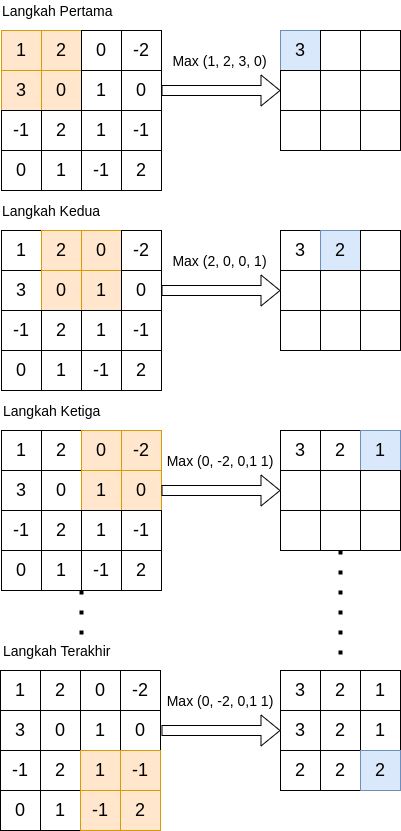
\includegraphics[scale=0.25]{gambar/max-pooling.png}
	\caption{Gambaran Proses \textit{Max Pooling}}
	\label{fig:max-pooling}
\end{figure}

\begin{equation}
	h'= \left[ \frac{h-f}{s} \right]
\end{equation}

\begin{equation}
	w'= \left[ \frac{w-f}{s} \right]
\end{equation}

Dimana $h'$ menunjukkan tinggi dari \textit{feature map output}, $w'$ menunjukkan lebar dari \textit{feature map output}, $h$ menunjukkan tinggi dari gambar \textit{input}, $w$ menunjukkan lebar dari gambar \textit{input}, $f$ adalah ukuran area \textit{pooling}, $s$ menunjukkan \textit{stride} operasi \textit{pooling}.

\subsection{Fungsi Aktivasi (\textit{Non-Linearity})}
\label{subsec:fungsi-aktivasi}

Tugas utama dari setiap fungsi aktivasi dalam setiap model berbasis jaringan saraf adalah untuk memetakan \textit{input output}, di mana nilai \textit{input} diperoleh dengan menghitung jumlah terbobot \textit{input neuron} dan selanjutnya menambahkan bias (jika ada bias). Dengan kata lain, fungsi aktivasi memutuskan apakah neuron akan aktif atau tidak untuk \textit{input} yang diberikan dengan menghasilkan \textit{output} yang sesuai. Terdapat beberapa fungsi aktivasi yang digunakan dalam CNN, antara lain :

\begin{enumerate}
	\item \textbf{Sigmoid}\\
	Fungsi aktivasi sigmoid mengambil bilangan real sebagai inputnya dan mengikat outputnya dalam kisaran [0,1]. Kurva fungsi sigmoid berbentuk 'S' seperti pada Gambar \ref{fig:sigmoid}. Representasi tematik dari sigmoid adalah:
	
	\begin{equation}
		f(x)_{sigm}=\frac{1}{1+e^{-x}}
	\end{equation}
	
	\begin{figure}[h!]
		\centering
		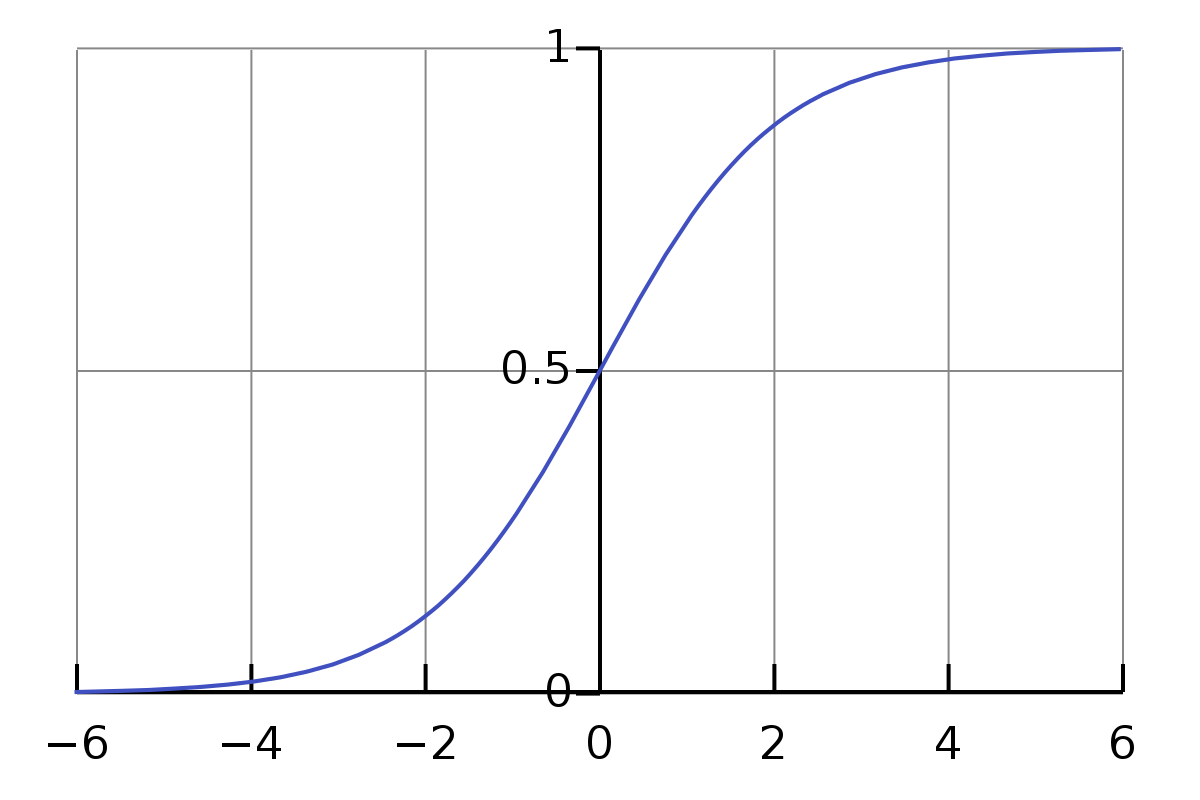
\includegraphics[scale=0.15]{gambar/sigmoid.png}
		\caption{Grafik Fungsi Aktivasi Sigmoid \citep{sigmoid}}
		\label{fig:sigmoid}
	\end{figure}
	
	\item \textbf{Tanh}\\
	Fungsi aktivasi Tanh digunakan untuk mengikat nilai input (bilangan real) dalam kisaran [-1,1] seperti tertampil pada Gambar \ref{fig:tanh}. Representasi matematis dari Tanh adalah:
	
	\begin{equation}
		f(x)_{tanh}=\frac{e^x-e^{-x}}{e^x+e^{-x}}
	\end{equation}
	
	
	\begin{figure}[h!]
		\centering
		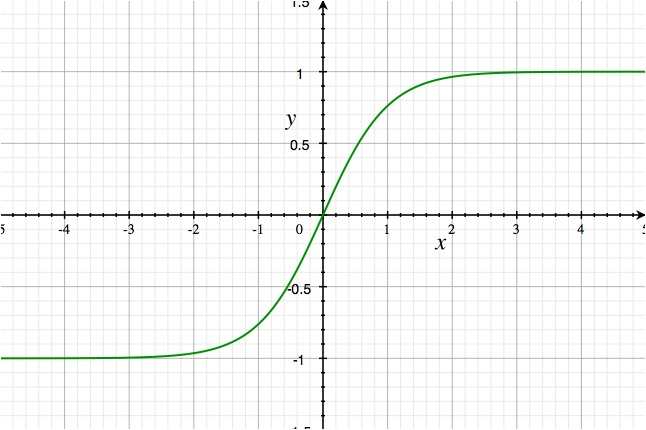
\includegraphics[scale=0.25]{gambar/tanh.jpg}
		\caption{Grafik Fungsi Aktivasi Tanh \citep{sigmoid}}
		\label{fig:tanh}
	\end{figure}
	
	\item \textbf{ReLU} \\
	Rectifier Linear Unit (ReLU) adalah fungsi aktivasi yang paling umum digunakan dalam Convolutional Neural Networks. Ini digunakan untuk mengubah semua nilai input menjadi bilangan positif. Keuntungan dari ReLU adalah membutuhkan beban komputasi yang sangat minimal dibandingkan dengan yang lain. Representasi matematis dari ReLU adalah:
	\begin{equation}
		f(x)_{ReLU}=\textbf{max}(0,x)
	\end{equation}
	
	Namun terkadang ada beberapa masalah besar dalam menggunakan fungsi aktivasi ReLU. Misalnya, jika terdapat gradient yang besar pada saat pencarian \textit{error} dengan menggunakan algortima \textit{back propagation}. Gradien yang besar ini apabila dilewatkan melalui fungsi ReLU, dapat menyebabkan bobot akan diperbarui sedemikian rupa sehingga neuron tidak pernah diaktifkan lagi. Masalah ini dikenal sebagai masalah \textit{"Dying ReLU"}. Untuk mengatasi masalah ini ada beberapa varian ReLU yang tersedia, diantaranya adalah Leaky ReLU dan Noisy ReLU. Tidak seperti ReLU, fungsi aktivasi Leaky ReLU tidak mengabaikan input negatif sepenuhnya, melainkan menurunkan skala input negatif tersebut. Leaky ReLU digunakan untuk menyelesaikan masalah \textit{Dying ReLU}. Representasi matematis dari Leaky ReLU adalah
	
	\begin{equation}
		f(x)_{LeakyReLU} =
		\begin{cases}
			x, & \text{if x$>$0}\\
			mx, & \text{if x$\leq$0}\\
		\end{cases}       
	\end{equation}  
	Di mana $m$ adalah konstanta, yang disebut faktor kebocoran dan umumnya disetel ke nilai kecil (seperti 0,001). Sedangkan Noisy ReLU digunakan distribusi Gaussian untuk membuat ReLU \textit{noisy}. Representasi matematis dari Noise ReLU adalah
	
	\begin{equation}
		f(x)_{NoisyReLU} = \textbf{max}(x + Y) , \textit{with} Y \sim N(0,\sigma(x))
	\end{equation}
	
\end{enumerate}

\subsection{Fully Connected Layer}
\label{subsec:fcn}

Biasanya bagian terakhir (atau lapisan) dari setiap arsitektur CNN (digunakan untuk klasifikasi) terdiri dari \textit{fully-connected layers}, di mana setiap neuron di dalam lapisan terhubung dengan setiap neuron dari lapisan sebelumnya. Lapisan terakhir dari lapisan \textit{Fully-Connected} digunakan sebagai lapisan keluaran (\textit{classifier}) dari arsitektur CNN. Lapisan \textit{Fully-Connected} adalah jenis jaringan saraf tiruan \textit{feed-forward} (ANN) dan mengikuti prinsip tradisional \textit{Multi-Layer Perceptron neural network} (MLP). Layer FC mengambil \textit{input} dari c\textit{onvolutional} atau \textit{pooling layer} akhir, yang berupa sekumpulan metrik (\textit{feature map}) dan matrik tersebut diratakan (\textit{flatten}) untuk membuat vektor dan vektor ini kemudian dimasukan ke dalam layer FC untuk menghasilkan hasil akhir \textit{output} CNN.

\subsection{\textit{Loss Function}}
\label{subsec:lossfunction}

Pada \textit{output layer}, dilakukan perhitungan kesalahan prediksi yang dihasilkan oleh model CNN atas sampel \textit{learning} menggunakan beberapa \textit{Loss Function}. \textit{Error} prediksi ini memberitahu jaringan bagaimana prediksinya dari \textit{output} aktual, dan kemudian \textit{error} ini akan dioptimalkan selama proses \textit{learning} model CNN. \textit{Loss function} menggunakan dua parameter untuk menghitung \textit{error}, parameter pertama adalah \textit{output} estimasi dari model CNN (juga disebut prediksi) dan yang kedua adalah \textit{output} aktual (juga dikenal sebagai label). Berikut adalah beberapa contoh \textit{loss function} yang banyak digunakan dalam algoritma \textit{deep learning}:


\begin{enumerate}
	\item \textit{\textbf{Cross-Entropy Loss Function}}\\
	\textit{Cross-entropy loss}, juga disebut fungsi \textit{log loss} banyak digunakan untuk mengukur kinerja model CNN, yang outputnya adalah probabilitas $p \in \{0,1\}$. \textit{Loss Function} ini banyak digunakan sebagai alternatif dari \textit{squared error loss function} dalam masalah klasifikasi multi-kelas. \textit{Cross-entropy loss} menggunakan aktivasi softmax di lapisan \textit{output} untuk menghasilkan \textit{output} dalam distribusi probabilitas, yaitu $p, y \in R^N$, di mana $p$ adalah probabilitas untuk setiap kategori \textit{output} dan $y$ menunjukkan \textit{output} yang diinginkan dan probabilitas setiap kelas \textit{output} dapat diperoleh dengan : 
	
	\begin{equation}
		p_i = \frac{e^{a_i}}{\sum_{k=1}^{N} e^{a_k}}
	\end{equation}
	
	Di mana $N$ adalah jumlah neuron di lapisan \textit{output} dan $e^{a_i}$ menunjukkan setiap \textit{output} yang tidak dinormalisasi dari lapisan sebelumnya dalam jaringan. Lalu, \textit{cross-entropy loss} dapat didefinisikan sebagai:
	
	\begin{equation}
		H(p,y) =-\sum_{i} y_i\log(p_i)
	\end{equation}
	\begin{center}
		dimana $i \in \left[1,N\right]$
	\end{center}
	
	\item \textbf{\textit{Euclidean Loss Function}}\\
	\textit{Euclidean Loss} juga disebut \textit{mean squared loss }banyak digunakan dalam masalah regresi. \textit{Mean squared loss} antara \textit{output} yang diprediksi $p \in R^N$ dan output aktual $y \in R^N$ di setiap neuron dari lapisan \textit{output} CNN didefinisikan sebagai :
	
	\begin{equation}
		H(p,y)=\frac{1}{2N} \sum_{i=1}^{N} (p_i-y_i)^2
	\end{equation}
	
	\item \textit{\textbf{Hinge Loss Function}}\\
	\textit{Hinge Loss} banyak digunakan dalam masalah klasifikasi biner. Ini digunakan dalam masalah klasifikasi berbasis "margin maksimum", terutama untuk \textit{support vector machine} (SVM). Di sini, \textit{optimizer} mencoba memaksimalkan margin antara dua kelas target. Hinge Loss Function didefinisikan sebagai:
	
	\begin{equation}
		H(p,y) = \sum_{i=1}^{N} \textbf{max}(0, m-(2y_i - 1)p_i)
	\end{equation}

	Dimana $m$ adalah margin yang biasanya bernilai sama dengan 1, dan $p_i$ menunjukkan prediksi \textit{output} dan $y_i$ menunjukkan output yang diinginkan
		
\end{enumerate}

\subsection{\textit{Regional-Based CNN}}
\label{subsec:rcnn}

Semenjak\textit{ Convolution Neural Network} (CNN) dengan \textit{fully connected layer} tidak mampu menangani frekuensi kemunculan dan multi objek. Salah satu cara untuk mengatasinya adalah dengan menggunakan \textit{sliding window brute force search} untuk memilih wilayah dan menerapkan model CNN pada area tersebut, tetapi masalah dari pendekatan ini adalah bahwa objek yang sama dapat direpresentasikan dalam gambar dengan ukuran dan aspek rasio yang berbeda. Dengan mempertimbangkan faktor-faktor tersebut, penerapan algoritma \textit{deep learning} (CNN) pada jumlah \textit{region proposal} yang banyak akan menyebabkan proses komputasi yang dijalankan akan menjadi sangat berat dan rumit.

\begin{figure}[h!]
	\centering
	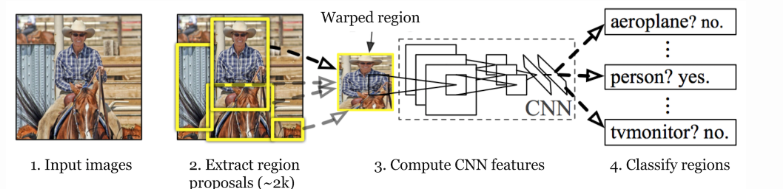
\includegraphics[scale=0.3]{gambar/rcnn.png}
	\caption{Arsitektur R-CNN \citep{arch-rcnn}}
	\label{fig:rcnn}
\end{figure}

Ross Girshick dan kawan-kawan pada tahun 2013 mengusulkan arsitektur baru yang disebut R-CNN seperti pada Gambar \ref{fig:rcnn} (\textit{Regional-based CNN}) untuk menghadapi tantangan deteksi objek ini \citep{rcnn}. Arsitektur R-CNN menggunakan algoritma \textit{selective search} yang menghasilkan sekitar 2000 \textit{region proposal}. \textit{Regional proposal} ini kemudian diterapkan ke arsitektur CNN untuk menghitung jumlah fitur CNN. Fitur-fitur ini kemudian diteruskan dalam model SVM untuk mengklasifikasikan objek yang ada di \textit{region proposal}. Langkah selanjutnya adalah melakukan regresi pada \textit{bounding box} untuk mengetahui lokasi objek yang ada dalam gambar dengan lebih tepat. 

\subsection{\textit{Fast R-CNN}}
\label{subsec:fast-rcnn}

Fast R-CNN ditemukan atas metode yang telah ditemukan terlebih dahulu yaitu \textit{R-CNN} untuk mengklasifikasikan proposal objek secara efisien menggunakan \textit{deep convolutional network} \citep{fast-rcnn}. Dibandingkan dengan \textit{R-CNN}, \textit{Fast R-CNN} menggunakan beberapa inovasi untuk meningkatkan kecepatan \textit{learning} dan pengujian sekaligus meningkatkan akurasi deteksi. Fast R-CNN dapat menyelesaikan proses \textit{training} dengan jaringan VGG16 yang sangat dalam memeberikan hasil yang 9 kali lebih cepat dari R-CNN, 213 kali lebih cepat pada waktu pengujian, dan mencapai mAP yang lebih tinggi pada PASCAL VOC 2012. Dibandingkan dengan SPPnet, Fast R-CNN dapat menyelesaikan proses \textit{training} dengan VGG16 3x lebih cepat, pengujian 10x lebih cepat, dan lebih akurat.

Jika pada R-CNN \textit{region proposal} akan melalui proses konvolusi di CNN, sebaliknya pada \textit{Fast R-CNN} gambar \textit{input}-lah yang akan melalui proses konvolusi di CNN seperti yang ditampilkan pada Gambar \ref{fig:fast-rcnn}. Hasil dari konvolusi pada \textit{Fast R-CNN} berupa \textit{convolutional feature map} yang akan digunakan untuk identifikasi \textit{region proposal} dan menyatukannya ke dalam bentuk persegi. Selanjutnya dengan menggunakan layer \textit{ROI Pooling} akan dibentuk kembali menjadi ukuran yang tetap sehingga dapat dimasukan ke dalam \textit{fully conneceted network}. Pada proses deteksi kelas dari \textit{region proposal} dan juga nilai offset dari \textit{bounding box} digunakan \textit{softmax layer} dari \textit{ROI feature vector} yang telah dihasilkan pada proses sebelumnya.

\begin{figure}[h]
	\centering
	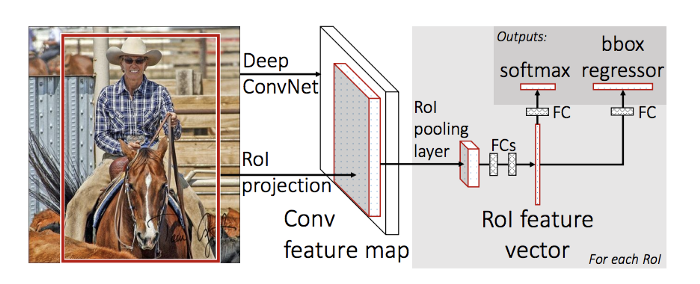
\includegraphics[scale=0.3]{gambar/fast-rcnn.png}
	\caption{Arsitektur \textit{Fast R-CNN} \citep{arch-fast-rcnn}}
	\label{fig:fast-rcnn}
\end{figure}

Alasan \textit{Fast R-CNN} lebih cepat daripada R-CNN adalah karena kita tidak perlu memasukkan 2000 \textit{region proposal} ke \textit{convolutional neural network} setiap saat. Sebagai gantinya, operasi konvolusi dilakukan hanya sekali per gambar dan \textit{feature map} dihasilkan operasi tersebut.

\subsection{\textit{Faster R-CNN}}
\label{subsec:faster-rcnn}

Pad kedua algoritma \textit{R-CNN} dan \textit{Fast R-CNN} menggunakan \textit{selective search} untuk mengetahui \textit{region proposal}. \textit{Selective search} sendiri memerlukan waktu yang cukup lama dalam penyelesain prosesnya sehingga mempengaruhi kinerja dari jaringan \citep{faster-rcnn}. Oleh karena itu, dibuatlah algoritma deteksi objek baru dengan menghilangkan algoritma \textit{selective search} dan memungkinkan jaringan mempelajari \textit{region proposal}.

Mirip dengan \textit{Fast R-CNN}, gambar dijadikann sebagai input ke jaringan konvolusi yang menyediakan \textit{convolusional feature map}. Disebabkan waktu eksekusi yang lama saat menggunakan algoritma \textit{selective search} pada \textit{feature map} untuk mengidentifikasi \textit{region proposal}, \textit{Faster R-CNN} menggunakan jaringan terpisah untuk memprediksi \textit{region proposal}. Jaringan terpisah ini dinamakan dengan \textit{Region Proposal Network (RPN)}, dimana \textit{RPN} berbagi \textit{full-image convolutional features} dengan jaringan deteksi yaitu \textit{Fast R-CNN}. \textit{Region proposal} yang diprediksi kemudian dibentuk kembali menggunakan \textit{ROI pooling layer} yang kemudian digunakan untuk mengklasifikasikan gambar di dalam \textit{region proposal} dan memprediksi nilai offset untuk \textit{bounding box}. Gambar \ref{fig:arch-faster-rcnn} merupakan visualisasi dari proses deteksi objek menggunakan \textit{Faster R-CNN}. 

\begin{figure}[h]
	\centering
	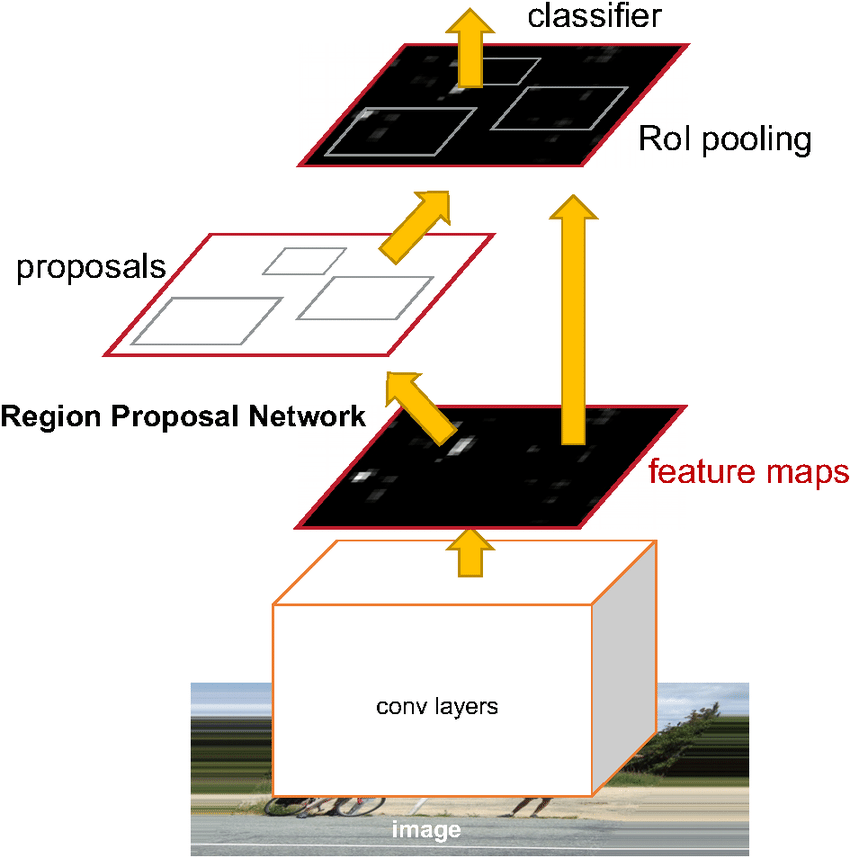
\includegraphics[scale=0.15]{gambar/arch-faster-rcnn.png}
	\caption{Gambaran Deteksi Objek pada \textit{Faster R-CNN} \citep{arch-faster-rcnn}}
	\label{fig:faster-rcnn}
\end{figure}

\subsection{\textit{Mask R-CNN}}
\label{subsec:mask-rcnn}

Mask R-CNN adalah Convolutional Neural Network (CNN) dan segmentasi citra termutakhir untuk saat ini. Varian Deep Neural Network ini mendeteksi objek dalam gambar dan menghasilkan \textit{mask} segmentasi berkualitas tinggi untuk setiap \textit{instance} \citep{mask-rcnn}. \textit{Mask R-CNN} dibangun menggunakan\textit{ Faster R-CNN} dimana \textit{Faster R-CNN} memiliki 2 \textit{output} untuk setiap objek, label kelas dan \textit{bounding box offset}. \textit{Mask R-CNN} adalah penambahan cabang ketiga yang mengeluarkan \textit{mask} objek seperti yang tertampil pada Gambar \ref{fig:arch-mask-rcnn}. \textit{output} \textit{mask} tambahan berbeda dari \textit{output} kelas dan \textit{bounding box}, yang membutuhkan ekstraksi tata letak spasial yang jauh lebih baik dari suatu objek.

\textit{Mask R-CNN} merupakan perpanjangan dari \textit{Faster R-CNN} dengan menambahkan cabang untuk memprediksi t\textit{mask} objek (\textit{Region of Interest}) secara paralel dengan cabang yang ada untuk pengenalan \textit{bounding box}. Satu keuntungan sederhana dari \textit{Mask R-CNN} dibandingkan \textit{Faster R-CNN} adalah kenyataan bahwa mudah untuk menggeneralisasi tugas lain seperti estimasi pose. Elemen kunci \textit{Mask R-CNN} adalah penyelarasan piksel-ke-piksel, yang merupakan bagian utama dari \textit{Fast/Faster R-CNN} yang hilang. \textit{Mask R-CNN} mengadopsi prosedur dua tahap yang sama dengan tahap pertama yang identik (yaitu \textit{RPN}). Pada tahap kedua, secara paralel untuk memprediksi kelas dan \textit{box offset}, Mask R-CNN juga mengeluarkan \textit{mask} biner untuk setiap \textit{RoI}. Ini berbeda dengan sistem terbaru, di mana klasifikasi bergantung pada prediksi \textit{mask}.

Mask R-CNN mudah diterapkan dan dilatih karena \textit{Faster R-CNN framework}, yang memfasilitasi berbagai desain arsitektur yang fleksibel. Selain itu, cabang \textit{mask} hanya menambahkan \textit{overhead} komputasi kecil, memungkinkan sistem dan eksperimen yang cepat.

\begin{figure}[h]
	\centering
	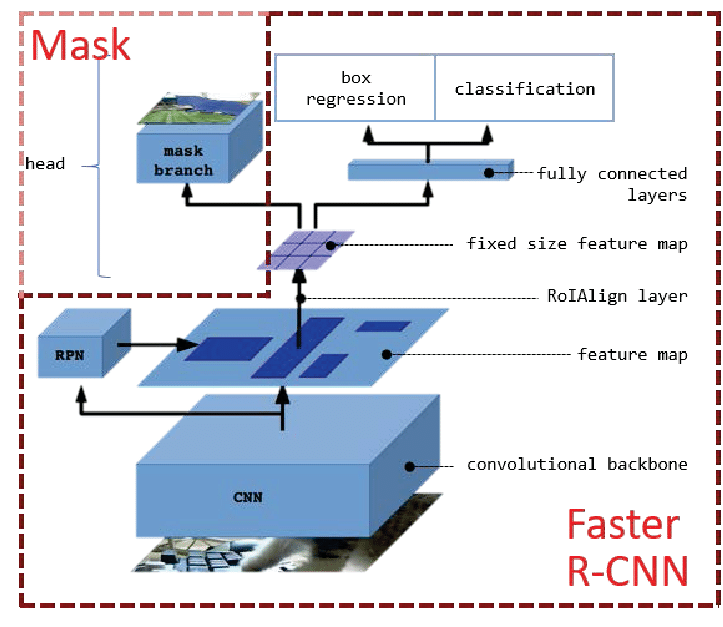
\includegraphics[scale=0.25]{gambar/arch-mask-rcnn.png}
	\caption{Struktur dari Arsitektur \textit{Faster R-CNN} \citep{arch-mask-rcnn}}
	\label{fig:mask-rcnn}
\end{figure}

\section{Penelitian Terkait}
\label{penelitianterkait}

\subsection{Real-Time Pedestrian Detection With Deep Network Cascades}
\label{realtime-pedestrian}

Penelitian ini dilakukan oleh Anelia Angelova dan kawan-kawan pada tahun 2015 yang menyajikan pendekatan real-time baru untuk deteksi objek yang mengeksploitasi efisiensi \textit{cascade classifiers} dengan akurasi \textit{deep neural network} \citep{penelitianterkait1}. \textit{Deep network} telah terbukti unggul dalam tugas klasifikasi, dan kemampuannya untuk beroperasi pada \textit{raw pixel input} tanpa perlu merancang fitur khusus. Namun, \textit{deep network} terkenal lambat pada waktu inferensi. Dalam \textit{paper} tersebut, Anelia Angelova dan kawan-kawan mengusulkan pendekatan \textit{cascades deep network} dan \textit{fast features}, yang sangat cepat dan sangat akurat. Mereka menerapkannya pada permasalahan pada deteksi pejalan kaki. Algoritma mereka berjalan secara real-time pada 15 frame per detik. Pendekatan yang dihasilkan mencapai tingkat kesalahan rata-rata 26,2\% pada \textit{benchmark} deteksi Caltech Pedestrian.

\subsection{Pedestrian Detection: The Elephant In The Room}
\label{pedestrian-detection}

Deteksi pejalan kaki digunakan di banyak aplikasi berbasis citra mulai dari pengawasan video hingga pengemudi otonom. Meskipun mencapai kinerja tinggi, sebagian besar masih belum diketahui seberapa baik detektor yang ada menggeneralisasi data yang tidak terlihat. Hal ini penting karena detektor yang praktis harus siap digunakan dalam berbagai skenario dalam aplikasi. Untuk tujuan tersebut, Irtiza Hasan dan kawan-kawan melakukan studi komprehensif dalam \textit{paper} ini, menggunakan prinsip umum evaluasi \textit{cross-dataset} langsung \citep{pedestrian-detection}. Melalui \textit{paper} ini, ditemukan bahwa detektor pejalan kaki terkini yang ada, meskipun berkinerja cukup baik ketika dilatih dan diuji pada kumpulan data yang sama, namun secara umum memiliki peforma yang cukup buruk dalam evaluasi \textit{cross-dataset}. 

Dalam \textit{paper} ini ditunjukkan bahwa ada dua alasan untuk permasalahan ini. Pertama, desain yang dibuat (misalnya, \textit{anchor settings}) mungkin bias terhadap tolok ukur dalam \textit{training} dan \textit{test pipeline} data tunggal, tetapi akibatnya sebagian besar membatasi kemampuan generalisasi dari keduanya. Kedua, sumber pelatihan umumnya tidak terlalu padat pada pejalan kaki dan mempunyi beragam dalam skenario. Di dalam evaluasi \textit{cross-dataset} langsung, secara mengejutkan, ditemukan bahwa detektor objek dengan tujuan umum, tanpa adaptasi khusus untuk pejalan kaki dalam desain, digeneralisasi jauh lebih baik dibandingkan dengan detektor pejalan kaki terkini yang ada. Lebih lanjut, diilustrasikan bahwa kumpulan data yang beragam dan padat, yang dikumpulkan dengan \textit{crawling web} , berfungsi sebagai sumber pra-pelatihan yang efisien untuk deteksi pejalan kaki. Oleh karena itu, pada \textit{paper} mengusulkan \textit{training pipelin} progresif dan menemukan bahwa \textit{pipeline} tersebut berfungsi dengan baik untuk deteksi pejalan kaki yang berorientasi pada pengemudian otonom. Akibatnya, studi yang dilakukan dalam makalah ini menunjukkan bahwa lebih banyak penekanan harus diberikan pada evaluasi \textit{cross-datasset} untuk desain masa mendatang pada detektor pejalan kaki.

\subsection{Fast Vehicle and Pedestrian Detection Using Improved Mask R-CNN}
\label{fast-vehicle}

Penelitian ini menyajikan algoritma Mask R-CNN yang sederhana dan efektif untuk deteksi kendaraan dan pejalan kaki yang lebih cepat \citep{fast-vehicle}. Metode ini memiliki nilai praktis untuk sistem peringatan anti-tabrakan dalam mengemudi cerdas. \textit{Deep Neural Network} dengan lebih banyak lapisan memiliki kapasitas yang lebih besar, tetapi juga harus melakukan perhitungan yang lebih rumit. Untuk mengatasi kelemahan ini, penelitian ini mengadopsi jaringan Resnet-86 sebagai \textit{backbone} yang berbeda dari struktur tulang punggung Resnet-101 dalam algoritma Mask R-CNN. Hasilnya menunjukkan bahwa jaringan Resnet-86 dapat mengurangi waktu operasi dan sangat meningkatkan akurasi. Kendaraan dan pejalan kaki yang terdeteksi juga disaring berdasarkan dataset Microsoft COCO. Dataset baru dibentuk dengan menyaring dan melengkapi COCO dataset, yang membuat pelatihan algoritma lebih efisien. Bagian terpenting dari penelitian ini adalah diusulkannya algoritma baru, \textit{Side Fusion FPN}. Parameter dalam algoritma tidak ada perubahan, jumlah perhitungan meningkat kurang dari 0,000001, dan rata-rata presisi (mAP) meningkat 2,00 poin. Hasilnya menunjukkan bahwa, dibandingkan dengan algoritma Mask R-CNN, algoritma pada penelitian ini menurunkan ukuran memori bobot sebesar 9,43\%, meningkatkan kecepatan pelatihan sebesar 26,98\%, meningkatkan kecepatan pengujian sebesar 7,94\%, menurunkan nilai \textit{error} sebesar 0,26, dan meningkatkan nilai mAP sebesar 17,53 poin.
  \cleardoublepage

  % Bab 3 desain dan implementasi
  \chapter{DESAIN DAN IMPLEMENTASI}
\label{chap:desainimplementasi}

% Ubah bagian-bagian berikut dengan isi dari desain dan implementasi

Penelitian ini dilaksanakan sesuai dengan sistem berikut dengan implementasinya. Desain sistem merupakan konsep dari pembuatan dan perancangan infrastruktur dan kemudian diwujud kan dalam bentuk blok-blok alur yang harus dikerjakan. Pada bagian implementasi merupakan pelaksanaan teknis untuk setiap blok pada desain sistem.

\section{Deskripsi Sistem}
\label{sec:deskripsisistem}

Sistem pada tugas akhir ini merupakan implementasi dari salah satu disiplin ilmu \textit{Deep Learning} dan pengolahan citra yang berfungsi untuk mendeteksi adanya pejalan kaki yang berada di pinggir jalan, trotoar dan jalur penyebrangan. Selain pejalan kaki, deteksi juga dilakukan pada jalur penyebrangan atau \textit{zebracross} dengan tujuan untuk memberi informasi bahwa disekitar area tersebut terdapat banyak aktivitas pejalan kaki yang menyebrang jalan. Blok diagram metodologi sistem yang digunakan pada penelitian ini dapat dilihat pada Gambar \ref{fig:blok-diagram}.

\begin{figure}[ht]
	\centering
	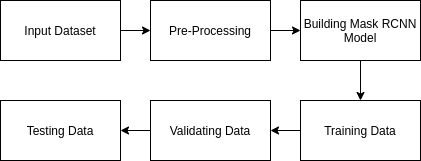
\includegraphics[scale=0.5]{gambar/blok-diagram.png}
	\caption{Blok Diagram Metodologi}
	\label{fig:blok-diagram}
\end{figure}  

\section{Pengumpulan \textit{Dataset} Gambar}
\label{sec:pengumpulandatagambar} 

Pada tugas akhir ini, \textit{dataset} yang digunakan didapatkan dengan beberapa cara, antara lain:
	\begin{enumerate}
		\item \textit{Caltech Pedestrian Database}, merupakan kumpulan gambar yang diambil dari sudut pandang pengendara mobil di California Amerika Serikat dengan ukuran 640 x 480 pixel. Terdapat sekitar 250.000 gambar dengan 350.000 \textit{bounding boxes} dan sekitar 2.300 pejalan kaki dengan kriteria unik diberi tanda. Namun, pada \textit{dataset} ini hanya pejalan kaki saja yang diberi label, sehingga perlu dilakukan proses pelabelan ulang sesuai kelas yang diinginkan. Tidak semua gambar pada \textit{dataset} ini diambil untuk digunakan, gambar yang mempunyai objek berupa pejalan kaki dan \textit{zebracross} saja yang akan digunakan. Gambar \ref{fig:caltech} merupakan contoh dari gambar yang terdapat pada \textit{Caltech Pedestrian Database}.
		\begin{figure}[ht]
			\centering
			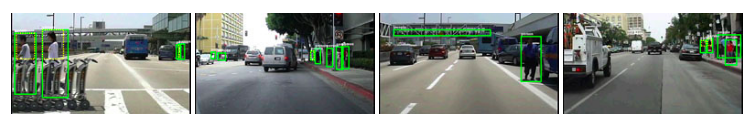
\includegraphics[scale=0.35]{gambar/caltech.png}
			\caption{Contoh Gambar dari Caltech Pedestrian Database}
			\label{fig:caltech}
		\end{figure} 
		
		\item Tangkapan layar dari beberapa video \textit{online Youtube}. Pada cara ini, penulis mencari video yang berada pada salah satu \textit{website video streaming} yaitu Youtube dengan persyaratan video diambil dari sudut pandang pengendara mobil yang berkendara pada jalan raya. Pada \textit{frame-frame} tertentu dilakukan \textit{screenshot} dan disimpan untuk selanjutnya dilakukan proses pemberian label pada objek-objek yang diinginkan seperti pada Gambar \ref{fig:youtube-dataset}. 
		
		\begin{figure}[ht]
			\centering
			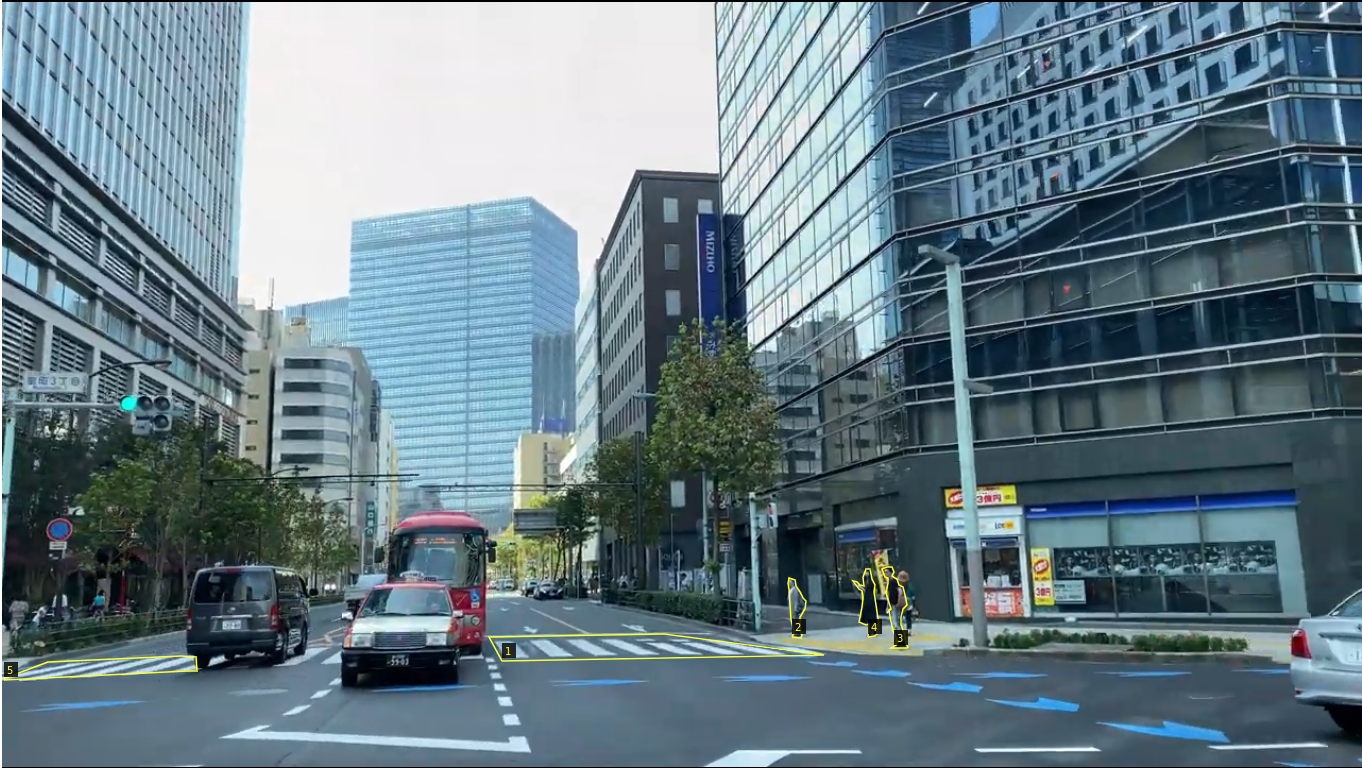
\includegraphics[scale=0.15]{gambar/youtube-dataset.png}
			\caption{Contoh Pembuatan \textit{dataset} dari \textit{Screenshot Youtube}}
			\label{fig:youtube-dataset}
		\end{figure}
		
		\item 
	\end{enumerate}

\section{Implementasi Alat
\label{sec:implementasi alat}}

Alat diimplementasikan dengan \lipsum[1]

% Contoh pembuatan potongan kode
\begin{lstlisting}[
  language=C++,
  caption={Program halo dunia.},
  label={lst:halodunia}
]
#include <iostream>

int main() {
    std::cout << "Halo Dunia!";
    return 0;
}
\end{lstlisting}

\lipsum[2-3]

% Contoh input potongan kode dari file
\lstinputlisting[
  language=Python,
  caption={Program perhitungan bilangan prima.},
  label={lst:bilanganprima}
]{program/bilangan-prima.py}

\lipsum[4]

  \cleardoublepage

  % Bab 4 pengujian dan analisis
  \chapter{PENGUJIAN DAN ANALISIS}
\label{chap:pengujiananalisis}

% Ubah bagian-bagian berikut dengan isi dari pengujian dan analisis

Pada bab ini dipaparkan hasil pengujian serta analisa dari desain sistem dan implementasi. Pengujian dilakukan guna mengetahui tingkat kesalahan dan menarik kesimpulan dari sistem yang telah dibuat.

Pada proses pengujian digunakan salah satu layanan \textit{Google} yaitu \textit{Google Colaboratory} dengan spesifikasi \textit{hardware} seperti pada Tabel \ref{tab:spek-colab}. Sedangkan untuk spesifikasi \textit{hardware} komputer penulis dapat dilihat pada Tabel \ref{tab:spek-pc}.
\begin{table}[h]
	\begin{center}
		\caption{Spesifikasi \textit{hardware Google Colaboratory}}
		\begin{tabular}{ |c|c| } 
			\hline
			\textbf{Procesor} & Intel Xeon Processor @ 2.3 GHz\\
			\hline 
			\textbf{Graphic Card} & Tesla K80 12 GB GDDR5 VRAM\\
			\hline 
			\textbf{RAM} & 16 GB\\ 
			\hline
		\end{tabular}
		\label{tab:spek-colab}
	\end{center}
\end{table} 

\begin{table}[h]
	\begin{center}
		\caption{Spesifikasi \textit{hardware} Komputer yang Digunakan}
		\begin{tabular}{ |c|c| } 
			\hline
			\textbf{Procesor} & Intel(R) Core(TM) i5-10400F CPU @ 2.90GHz\\
			\hline 
			\textbf{Graphic Card} & Nvidia GeForce GTX 1650 4 GB GDDR6\\
			\hline 
			\textbf{RAM} & 8 GB\\ 
			\hline
		\end{tabular}
		\label{tab:spek-pc}
	\end{center}
\end{table}

Pengujian dilakukan dengan membagi model ke beberapa jenis \textit{backbone} yang digunakan, antara lain Resnet-50, Resnet-101, dan Mobilenet-V1.

\section{Pengujian Jenis \textit{Backbone}}
\label{sec:pengujian-backbone}

Pengujian pada jenis \textit{backbone} bertujuan untuk mengetahui performa dan akurasi dari setiap model yang dihasilkan dengan \textit{backbone} yang berbeda.

\subsection{Resnet-50}
\label{subsec:resnet50}

Tabel \ref{tab:conf-resnet50} merupakan parameter-parameter yang digunakan untuk membuat model Mask R-CNN dengan menggunakan \textit{backbone} Resnet-50.

% Please add the following required packages to your document preamble:
% \usepackage{longtable}
% Note: It may be necessary to compile the document several times to get a multi-page table to line up properly
\begin{longtable}[h]{|l|l|}
	\caption{Konfigurasi Model menggunakan Resnet-50}
	\label{tab:conf-resnet50}\\
	\hline
	\multicolumn{2}{|c|}{\textbf{Pengaturan Model Resnet-50}}                                                                                                                                                                \\ \hline
	\endfirsthead
	%
	\multicolumn{2}{c}%
	{{\tablename\ \thetable{} -- Lanjutan dari halaman sebelumnya}} \\
	\endhead
	%
	\multicolumn{2}{|r|}{\textit{Dilanjutkan pada halaman berikutnya}} \\ \hline
	\endfoot
	%
	\endlastfoot
	BACKBONE                        & resnet50                                                                                                                                                                               \\ \hline
	BACKBONE\_STRIDES               & {[}4, 8, 16, 32, 64{]}                                                                                                                                                                 \\ \hline
	BATCH\_SIZE                     & 1                                                                                                                                                                                      \\ \hline
	BBOX\_STD\_DEV                  & {[}0.1 0.1 0.2 0.2{]}                                                                                                                                                                  \\ \hline
	COMPUTE\_BACKBONE\_SHAPE        & None                                                                                                                                                                                   \\ \hline
	DETECTION\_MAX\_INSTANCES       & 50                                                                                                                                                                                     \\ \hline
	DETECTION\_MIN\_CONFIDENCE      & 0.9                                                                                                                                                                                    \\ \hline
	DETECTION\_NMS\_THRESHOLD       & 0.2                                                                                                                                                                                    \\ \hline
	FPN\_CLASSIF\_FC\_LAYERS\_SIZE  & 1024                                                                                                                                                                                   \\ \hline
	GPU\_COUNT                      & 1                                                                                                                                                                                      \\ \hline
	GRADIENT\_CLIP\_NORM            & 5.0                                                                                                                                                                                    \\ \hline
	IMAGES\_PER\_GPU                & 1                                                                                                                                                                                      \\ \hline
	IMAGE\_CHANNEL\_COUNT           & 3                                                                                                                                                                                      \\ \hline
	IMAGE\_MAX\_DIM                 & 512                                                                                                                                                                                    \\ \hline
	IMAGE\_META\_SIZE               & 16                                                                                                                                                                                     \\ \hline
	IMAGE\_MIN\_DIM                 & 400                                                                                                                                                                                    \\ \hline
	IMAGE\_MIN\_SCALE               & 0                                                                                                                                                                                      \\ \hline
	IMAGE\_RESIZE\_MODE             & square                                                                                                                                                                                 \\ \hline
	IMAGE\_SHAPE                    & {[}512 512 3{]}                                                                                                                                                                        \\ \hline
	LEARNING\_MOMENTUM              & 0.9                                                                                                                                                                                    \\ \hline
	LEARNING\_RATE                  & 0.001                                                                                                                                                                                  \\ \hline
	LOSS\_WEIGHTS                   & \begin{tabular}[c]{@{}l@{}}\{'rpn\_class\_loss': 1.0,\\  'rpn\_bbox\_loss': 1.0, \\ 'mrcnn\_class\_loss': 1.0, \\ 'mrcnn\_bbox\_loss': 1.0, \\ 'mrcnn\_mask\_loss': 1.0\}\end{tabular} \\ \hline
	MASK\_POOL\_SIZE                & 14                                                                                                                                                                                     \\ \hline
	MASK\_SHAPE                     & {[}28, 28{]}                                                                                                                                                                           \\ \hline
	MAX\_GT\_INSTANCES              & 50                                                                                                                                                                                     \\ \hline
	MEAN\_PIXEL                     & {[}123.7 116.8 103.9{]}                                                                                                                                                                \\ \hline
	MINI\_MASK\_SHAPE               & (56, 56)                                                                                                                                                                               \\ \hline
	NAME                            & object                                                                                                                                                                                 \\ \hline
	NUM\_CLASSES                    & 4                                                                                                                                                                                      \\ \hline
	POOL\_SIZE                      & 7                                                                                                                                                                                      \\ \hline
	POST\_NMS\_ROIS\_INFERENCE      & 1000                                                                                                                                                                                   \\ \hline
	POST\_NMS\_ROIS\_TRAINING       & 2000                                                                                                                                                                                   \\ \hline
	PRE\_NMS\_LIMIT                 & 6000                                                                                                                                                                                   \\ \hline
	ROI\_POSITIVE\_RATIO            & 0.33                                                                                                                                                                                   \\ \hline
	RPN\_ANCHOR\_RATIOS             & {[}0.5, 1, 2{]}                                                                                                                                                                        \\ \hline
	RPN\_ANCHOR\_SCALES             & (32, 64, 128, 256, 512)                                                                                                                                                                \\ \hline
	RPN\_ANCHOR\_STRIDE             & 1                                                                                                                                                                                      \\ \hline
	RPN\_BBOX\_STD\_DEV             & {[}0.1 0.1 0.2 0.2{]}                                                                                                                                                                  \\ \hline
	RPN\_NMS\_THRESHOLD             & 0.7                                                                                                                                                                                    \\ \hline
	RPN\_TRAIN\_ANCHORS\_PER\_IMAGE & 256                                                                                                                                                                                    \\ \hline
	STEPS\_PER\_EPOCH               & 100                                                                                                                                                                                    \\ \hline
	TOP\_DOWN\_PYRAMID\_SIZE        & 256                                                                                                                                                                                    \\ \hline
	TRAIN\_BN                       & False                                                                                                                                                                                  \\ \hline
	TRAIN\_ROIS\_PER\_IMAGE         & 200                                                                                                                                                                                    \\ \hline
	USE\_MINI\_MASK                 & True                                                                                                                                                                                   \\ \hline
	USE\_RPN\_ROIS                  & True                                                                                                                                                                                   \\ \hline
	VALIDATION\_STEPS               & 30                                                                                                                                                                                     \\ \hline
	WEIGHT\_DECAY                   & 0.0001
	\\ \hline                 
\end{longtable}

Setelah dilakukan serangkaian proses training yang memakan waktu sekitar 3 jam 40 menit 24 detik didapatkan \textit{output} berupa \textit{model file}  dengan format \textit{h5} yang mempunyai ukuran 170.9 MB. \textit{Training loss} terendah yang berhasil dicapai dengan menggunakan \textit{backbone} Resnet-50 (pada \textit{epoch} ke 242) adalah 0.4061 dengan rincian \textit{training bounding box loss} sebesar 0.04083, \textit{training classification loss} sebesar 0.02268 serta \textit{training mask loss} sebesar 0.139 (dimana $L=L_{bbox}+L_{cls}+L_{mask}$). Gambar \ref{fig:resnet50-training} merupakan grafik yang menunjukkan perubahan \textit{training loss, training bounding box loss, training classification loss,} serta \textit{training mask loss} dari \textit{epoch} 1 sampai 300.

\begin{figure}[H]
	\centering
	\begin{minipage}{0.45\textwidth}
		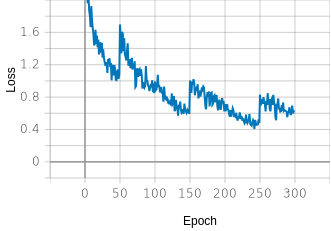
\includegraphics[width=\textwidth]{gambar/training_resnet50/tugas-akhir-Page-12.png}
		\caption*{(a) \textit{Training Loss}}
	\end{minipage}
	\hfill
	\begin{minipage}{0.45\textwidth}
		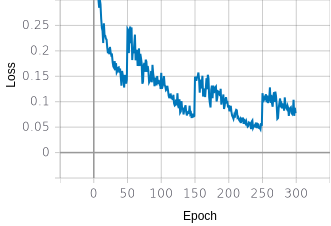
\includegraphics[width=\textwidth]{gambar/training_resnet50/tugas-akhir-Page-12-(1).png}
		\caption*{(b) \textit{Training Bounding Box Loss}}
	\end{minipage}
	\vfill
	\begin{minipage}{0.45\textwidth}
		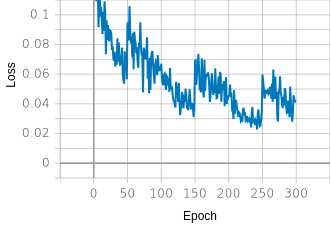
\includegraphics[width=\textwidth]{gambar/training_resnet50/tugas-akhir-Page-12-(2).png}
		\caption*{(c) \textit{Training Classification Loss}}
	\end{minipage}
	\hfill
	\begin{minipage}{0.45\textwidth}
		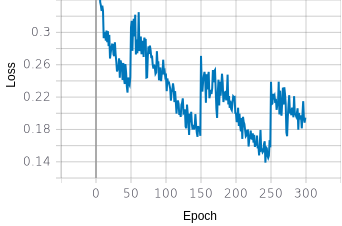
\includegraphics[width=\textwidth]{gambar/training_resnet50/tugas-akhir-Page-12-(3).png}
		\caption*{(d) \textit{Training Mask Loss}}
	\end{minipage}
	\caption{Grafik Perubahan \textit{Training Loss} pada \textit{Resnet-50}}
	\label{fig:resnet50-training}
\end{figure}

Sedangkan pada saat proses \textit{validation} sendiri \textit{Loss} terendah yang berhasil dicapai pada \textit{epoch} ke 266 dengan nilai sebesar 0.3653 dengan rincian \textit{validation bounding box loss} sebesar 0.4556, \textit{validation classification loss} sebesar 0.01912 serta \textit{validation mask loss} sebesar 0.1519. Namun untuk \textit{validation bounding box loss} terendah berada pada \textit{epoch} ke 260 dengan nilai sebesar 0.4203 sedangkan \textit{validation classification loss} terendah pada \textit{epoch} ke 210 dengan nilai 0.01525 serta \textit{validation mask loss} terendah pada \textit{epoch} ke 201 dengan nilai 0.1439. Gambar \ref{fig:resnet50-val} merupakan grafik yang menunjukkan perubahan \textit{validation loss, validation bounding box loss, validation classification loss,} serta \textit{validation mask loss} dari \textit{epoch} 1 sampai 300.

\begin{figure}[H]
	\centering
	\begin{minipage}{0.45\textwidth}
		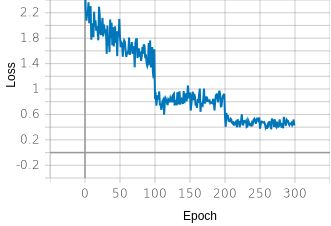
\includegraphics[width=\textwidth]{gambar/training_resnet50/tugas-akhir-Page-13.png}
		\caption*{(a) \textit{Validation Loss}}
	\end{minipage}
	\hfill
	\begin{minipage}{0.45\textwidth}
		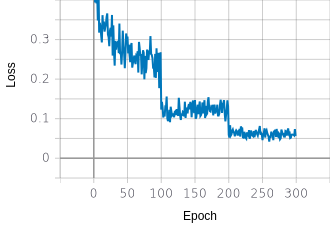
\includegraphics[width=\textwidth]{gambar/training_resnet50/tugas-akhir-Page-13 (1).png}
		\caption*{(b) \textit{Validation Bounding Box Loss}}
	\end{minipage}
	\vfill
	\begin{minipage}{0.45\textwidth}
		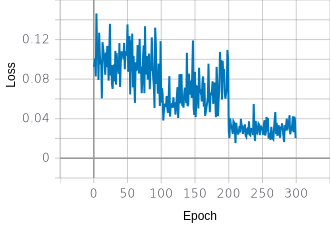
\includegraphics[width=\textwidth]{gambar/training_resnet50/tugas-akhir-Page-13 (2).png}
		\caption*{(c) \textit{Validation Classification Loss}}
	\end{minipage}
	\hfill
	\begin{minipage}{0.45\textwidth}
		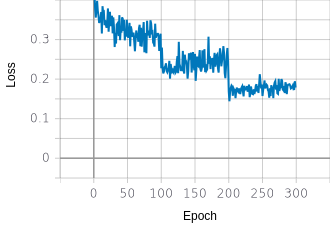
\includegraphics[width=\textwidth]{gambar/training_resnet50/tugas-akhir-Page-13 (3).png}
		\caption*{(d) \textit{Validation Mask Loss}}
	\end{minipage}
	\caption{Grafik Perubahan \textit{Validation Loss} pada \textit{Resnet-50}}
	\label{fig:resnet50-val}
\end{figure}

Selain menggunakan \textit{Loss Function} untuk mengukur peforma hasil \textit{training} yang sudah dilakukan, digunakan juga \textit{mean Average Precision (mAP)}. \textit{Precision} sendiri merupakan fungsi untuk menggambarkan tingkat keakuratan antara data yang diminta dengan hasil prediksi yang diberikan oleh model. Maka, \textit{precision} merupakan rasio prediksi benar positif (TP) dibandingkan dengan keseluruhan hasil yang diprediksi positif (TP dan FP). Rumus untuk mencari \textit{Precision} adalah sebagai berikut :
\begin{equation}
	Precision = \frac{TP}{TP+FP} 
\end{equation}

Perhitungan \textit{mAP} pada penelitian ini dilakukan setiap 5 \textit{epoch} sekali, karena jika dilakukan setiap \textit{epoch} akan memerlukan \textit{training time} yang lebih lama serta \textit{resource hardware} yang diperlukan lebih besar. Nilai \textit{mAP} tertinggi didapatkan pada \textit{epoch} ke 220 sebesar 94.92. Gambar \ref{fig:resnet50-map} merupakan grafik yang menunjukan perubahan \textit{validation mean Average Precision} dari \textit{epoch} 1 sampai 300. 

\begin{figure}[H]
	\centering
	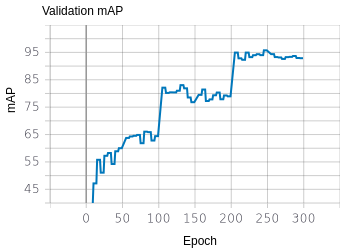
\includegraphics[scale=0.4]{gambar/resnet50-map.png}
	\caption{Grafik Perubahan \textit{Validation mAP} pada Resnet-50}
	\label{fig:resnet50-map}
\end{figure}

\subsection{Resnet-101}
\label{subsec:resnet101}

Tabel \ref{tab:conf-resnet101} merupakan parameter-parameter yang digunakan untuk membuat model Mask R-CNN dengan menggunakan \textit{backbone} Resnet-101.

% Please add the following required packages to your document preamble:
% \usepackage{longtable}
% Note: It may be necessary to compile the document several times to get a multi-page table to line up properly
\begin{longtable}{|l|l|}
	\caption{Konfigurasi Model menggunakan Resnet-101}
	\label{tab:conf-resnet101}\\
	\hline
	\multicolumn{2}{|c|}{\textbf{Pengaturan Model Resnet-101}}                                                                                                                                                             \\ \hline
	\endfirsthead
	%
	\multicolumn{2}{c}%
	{{\tablename\ \thetable{} -- Lanjutan dari halaman sebelumnya}} \\
	\endhead
	%
	\multicolumn{2}{|r|}{\textit{Dilanjutkan pada halaman berikutnya}} \\ \hline
	\endfoot
	%
	\endlastfoot
	BACKBONE                        & resnet101                                                                                                                                                                            \\ \hline
	BACKBONE\_STRIDES               & {[}4, 8, 16, 32, 64{]}                                                                                                                                                                 \\ \hline
	BATCH\_SIZE                     & 1                                                                                                                                                                                      \\ \hline
	BBOX\_STD\_DEV                  & {[}0.1 0.1 0.2 0.2{]}                                                                                                                                                                  \\ \hline
	COMPUTE\_BACKBONE\_SHAPE        & None                                                                                                                                                                                   \\ \hline
	DETECTION\_MAX\_INSTANCES       & 50                                                                                                                                                                                     \\ \hline
	DETECTION\_MIN\_CONFIDENCE      & 0.9                                                                                                                                                                                    \\ \hline
	DETECTION\_NMS\_THRESHOLD       & 0.2                                                                                                                                                                                    \\ \hline
	FPN\_CLASSIF\_FC\_LAYERS\_SIZE  & 1024                                                                                                                                                                                   \\ \hline
	GPU\_COUNT                      & 1                                                                                                                                                                                      \\ \hline
	GRADIENT\_CLIP\_NORM            & 5.0                                                                                                                                                                                    \\ \hline
	IMAGES\_PER\_GPU                & 1                                                                                                                                                                                      \\ \hline
	IMAGE\_CHANNEL\_COUNT           & 3                                                                                                                                                                                      \\ \hline
	IMAGE\_MAX\_DIM                 & 512                                                                                                                                                                                    \\ \hline
	IMAGE\_META\_SIZE               & 16                                                                                                                                                                                     \\ \hline
	IMAGE\_MIN\_DIM                 & 400                                                                                                                                                                                    \\ \hline
	IMAGE\_MIN\_SCALE               & 0                                                                                                                                                                                      \\ \hline
	IMAGE\_RESIZE\_MODE             & square                                                                                                                                                                                 \\ \hline
	IMAGE\_SHAPE                    & {[}512 512 3{]}                                                                                                                                                                        \\ \hline
	LEARNING\_MOMENTUM              & 0.9                                                                                                                                                                                    \\ \hline
	LEARNING\_RATE                  & 0.001                                                                                                                                                                                  \\ \hline
	LOSS\_WEIGHTS                   & \begin{tabular}[c]{@{}l@{}}\{'rpn\_class\_loss': 1.0,\\  'rpn\_bbox\_loss': 1.0, \\ 'mrcnn\_class\_loss': 1.0, \\ 'mrcnn\_bbox\_loss': 1.0, \\ 'mrcnn\_mask\_loss': 1.0\}\end{tabular} \\ \hline
	MASK\_POOL\_SIZE                & 14                                                                                                                                                                                     \\ \hline
	MASK\_SHAPE                     & {[}28, 28{]}                                                                                                                                                                           \\ \hline
	MAX\_GT\_INSTANCES              & 50                                                                                                                                                                                     \\ \hline
	MEAN\_PIXEL                     & {[}123.7 116.8 103.9{]}                                                                                                                                                                \\ \hline
	MINI\_MASK\_SHAPE               & (56, 56)                                                                                                                                                                               \\ \hline
	NAME                            & object                                                                                                                                                                                 \\ \hline
	NUM\_CLASSES                    & 4                                                                                                                                                                                      \\ \hline
	POOL\_SIZE                      & 7                                                                                                                                                                                      \\ \hline
	POST\_NMS\_ROIS\_INFERENCE      & 1000                                                                                                                                                                                   \\ \hline
	POST\_NMS\_ROIS\_TRAINING       & 2000                                                                                                                                                                                   \\ \hline
	PRE\_NMS\_LIMIT                 & 6000                                                                                                                                                                                   \\ \hline
	ROI\_POSITIVE\_RATIO            & 0.33                                                                                                                                                                                   \\ \hline
	RPN\_ANCHOR\_RATIOS             & {[}0.5, 1, 2{]}                                                                                                                                                                        \\ \hline
	RPN\_ANCHOR\_SCALES             & (32, 64, 128, 256, 512)                                                                                                                                                                \\ \hline
	RPN\_ANCHOR\_STRIDE             & 1                                                                                                                                                                                      \\ \hline
	RPN\_BBOX\_STD\_DEV             & {[}0.1 0.1 0.2 0.2{]}                                                                                                                                                                  \\ \hline
	RPN\_NMS\_THRESHOLD             & 0.7                                                                                                                                                                                    \\ \hline
	RPN\_TRAIN\_ANCHORS\_PER\_IMAGE & 256                                                                                                                                                                                    \\ \hline
	STEPS\_PER\_EPOCH               & 100                                                                                                                                                                                    \\ \hline
	TOP\_DOWN\_PYRAMID\_SIZE        & 256                                                                                                                                                                                    \\ \hline
	TRAIN\_BN                       & False                                                                                                                                                                                  \\ \hline
	TRAIN\_ROIS\_PER\_IMAGE         & 200                                                                                                                                                                                    \\ \hline
	USE\_MINI\_MASK                 & True                                                                                                                                                                                   \\ \hline
	USE\_RPN\_ROIS                  & True                                                                                                                                                                                   \\ \hline
	VALIDATION\_STEPS               & 30                                                                                                                                                                                     \\ \hline
	WEIGHT\_DECAY                   & 0.0001                                                                                                                                                                                 \\ \hline
\end{longtable}

Setelah dilakukan serangkaian proses training yang memakan waktu sekitar 4 jam 9 menit 16 detik didapatkan \textit{output} berupa \textit{model file}  dengan format \textit{h5} yang mempunyai ukuran 244 MB. \textit{Training loss} terendah yang berhasil dicapai dengan menggunakan \textit{backbone} Resnet-101 (pada \textit{epoch} ke 244) adalah 0.3933 dengan rincian \textit{training bounding box loss} sebesar 0.04164, \textit{training classification loss} sebesar 0.0247 serta \textit{training mask loss} sebesar 0.1403. Namun untuk \textit{training bounding box loss} terendah terdapat pada \textit{epoch} ke 246 dengan nilai sebesar 0.04083, \textit{training classification loss} terendah pada \textit{epoch} ke 234 dengan nilai 0.01957. Gambar \ref{fig:resnet101-training} merupakan grafik yang menunjukkan perubahan \textit{training loss, training bounding box loss, training classification loss,} serta \textit{training mask loss} dari \textit{epoch} 1 sampai 300. 

\newpage

\begin{figure}[H]
	\centering
	\begin{minipage}{0.45\textwidth}
		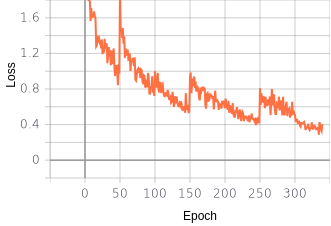
\includegraphics[width=\textwidth]{gambar/training_resnet50/tugas-akhir-Page-15.png}
		\caption*{(a) \textit{Training Loss}}
	\end{minipage}
	\hfill
	\begin{minipage}{0.45\textwidth}
		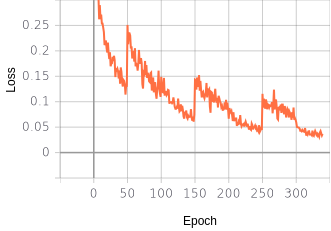
\includegraphics[width=\textwidth]{gambar/training_resnet50/tugas-akhir-Page-15 (1).png}
		\caption*{(b) \textit{Training Bounding Box Loss}}
	\end{minipage}
	\vfill
	\begin{minipage}{0.45\textwidth}
		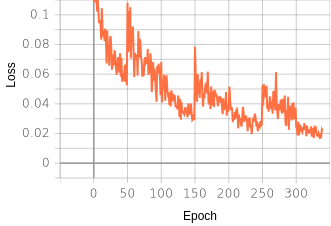
\includegraphics[width=\textwidth]{gambar/training_resnet50/tugas-akhir-Page-15 (2).png}
		\caption*{(c) \textit{Training Classification Loss}}
	\end{minipage}
	\hfill
	\begin{minipage}{0.45\textwidth}
		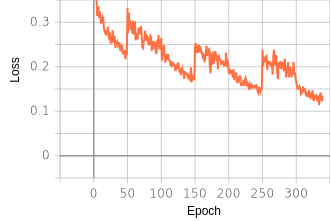
\includegraphics[width=\textwidth]{gambar/training_resnet50/tugas-akhir-Page-15 (3).png}
		\caption*{(d) \textit{Training Mask Loss}}
	\end{minipage}
	\caption{Grafik Perubahan \textit{Training Loss} pada \textit{Resnet-101}}
	\label{fig:resnet101-training}
\end{figure}

Sedangkan pada saat proses \textit{validation} sendiri \textit{Loss} terendah yang berhasil dicapai pada \textit{epoch} ke 266 dengan nilai sebesar 0.299 dengan rincian \textit{validation bounding box loss} sebesar 0.03867, \textit{validation classification loss} sebesar 0.01246 serta \textit{validation mask loss} sebesar 0.1461. Gambar \ref{fig:resnet101-val} merupakan grafik yang menunjukkan perubahan \textit{validation loss, validation bounding box loss, validation classification loss,} serta \textit{validation mask loss} dari \textit{epoch} 1 sampai 300.

\newpage

\begin{figure}[H]
	\centering
	\begin{minipage}{0.45\textwidth}
		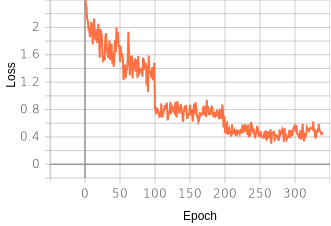
\includegraphics[width=\textwidth]{gambar/training_resnet50/tugas-akhir-Page-16.png}
		\caption*{(a) \textit{Validation Loss}}
	\end{minipage}
	\hfill
	\begin{minipage}{0.45\textwidth}
		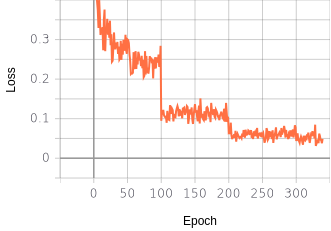
\includegraphics[width=\textwidth]{gambar/training_resnet50/tugas-akhir-Page-16 (1).png}
		\caption*{(b) \textit{Validation Bounding Box Loss}}
	\end{minipage}
	\vfill
	\begin{minipage}{0.45\textwidth}
		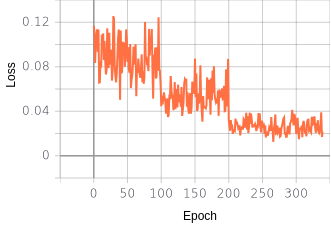
\includegraphics[width=\textwidth]{gambar/training_resnet50/tugas-akhir-Page-16 (2).png}
		\caption*{(c) \textit{Validation Classification Loss}}
	\end{minipage}
	\hfill
	\begin{minipage}{0.45\textwidth}
		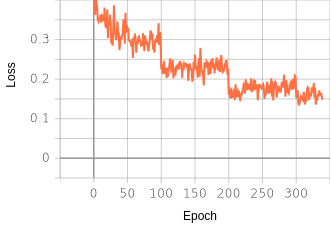
\includegraphics[width=\textwidth]{gambar/training_resnet50/tugas-akhir-Page-16 (3).png}
		\caption*{(d) \textit{Validation Mask Loss}}
	\end{minipage}
	\caption{Grafik Perubahan \textit{Validation Loss} pada \textit{Resnet-101}}
	\label{fig:resnet101-val}
\end{figure}

Nilai \textit{mAP} tertinggi didapatkan pada \textit{epoch} ke 215 sebesar 96.21. Gambar \ref{fig:resnet101-map} merupakan grafik yang menunjukan perubahan \textit{validation mean Average Precision} dari \textit{epoch} 1 sampai 300.

\begin{figure}[h]
	\centering
	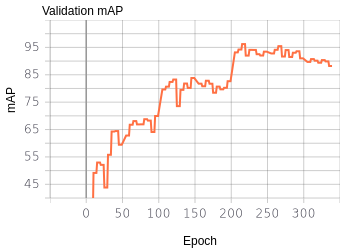
\includegraphics[scale=0.4]{gambar/resnet101-map.png}
	\caption{Grafik Perubahan \textit{Validation mAP} pada \textit{Resnet-101}}
	\label{fig:resnet101-map}
\end{figure} 

\subsection{MobileNet-V1}
\label{subsec:mobilenetv1}

Tabel \ref{tab:conf-mobilenet-v1} merupakan parameter-parameter yang digunakan untuk membuat model Mask R-CNN dengan menggunakan \textit{backbone} Mobilenet-V1.

% Please add the following required packages to your document preamble:
% \usepackage{longtable}
% Note: It may be necessary to compile the document several times to get a multi-page table to line up properly
\begin{longtable}[h]{|l|l|}
	\caption{Konfigurasi Model menggunakan Mobilenet-V1}
	\label{tab:conf-mobilenet-v1}\\
	\hline
	\multicolumn{2}{|c|}{\textbf{Pengaturan Model Mobilenet-V1}}                                                                                                                                                             
	\\ \hline
	\endfirsthead
	%
	\multicolumn{2}{c}%
	{{\tablename\ \thetable{} -- Lanjutan dari halaman sebelumnya}} \\
	\endhead
	%
	\multicolumn{2}{|r|}{\textit{Dilanjutkan pada halaman berikutnya}} \\ \hline
	\endfoot
	%
	\endlastfoot
	BACKBONE                        & mobilenetv1                                                                                                                                                                            \\ \hline
	BACKBONE\_STRIDES               & {[}4, 8, 16, 32, 64{]}                                                                                                                                                                 \\ \hline
	BATCH\_SIZE                     & 1                                                                                                                                                                                      \\ \hline
	BBOX\_STD\_DEV                  & {[}0.1 0.1 0.2 0.2{]}                                                                                                                                                                  \\ \hline
	COMPUTE\_BACKBONE\_SHAPE        & None                                                                                                                                                                                   \\ \hline
	DETECTION\_MAX\_INSTANCES       & 50                                                                                                                                                                                     \\ \hline
	DETECTION\_MIN\_CONFIDENCE      & 0.9                                                                                                                                                                                    \\ \hline
	DETECTION\_NMS\_THRESHOLD       & 0.2                                                                                                                                                                                    \\ \hline
	FPN\_CLASSIF\_FC\_LAYERS\_SIZE  & 1024                                                                                                                                                                                   \\ \hline
	GPU\_COUNT                      & 1                                                                                                                                                                                      \\ \hline
	GRADIENT\_CLIP\_NORM            & 5.0                                                                                                                                                                                    \\ \hline
	IMAGES\_PER\_GPU                & 1                                                                                                                                                                                      \\ \hline
	IMAGE\_CHANNEL\_COUNT           & 3                                                                                                                                                                                      \\ \hline
	IMAGE\_MAX\_DIM                 & 512                                                                                                                                                                                    \\ \hline
	IMAGE\_META\_SIZE               & 16                                                                                                                                                                                     \\ \hline
	IMAGE\_MIN\_DIM                 & 400                                                                                                                                                                                    \\ \hline
	IMAGE\_MIN\_SCALE               & 0                                                                                                                                                                                      \\ \hline
	IMAGE\_RESIZE\_MODE             & square                                                                                                                                                                                 \\ \hline
	IMAGE\_SHAPE                    & {[}512 512 3{]}                                                                                                                                                                        \\ \hline
	LEARNING\_MOMENTUM              & 0.9                                                                                                                                                                                    \\ \hline
	LEARNING\_RATE                  & 0.001                                                                                                                                                                                  \\ \hline
	LOSS\_WEIGHTS                   & \begin{tabular}[c]{@{}l@{}}\{'rpn\_class\_loss': 1.0,\\  'rpn\_bbox\_loss': 1.0, \\ 'mrcnn\_class\_loss': 1.0, \\ 'mrcnn\_bbox\_loss': 1.0, \\ 'mrcnn\_mask\_loss': 1.0\}\end{tabular} \\ \hline
	MASK\_POOL\_SIZE                & 14                                                                                                                                                                                     \\ \hline
	MASK\_SHAPE                     & {[}28, 28{]}                                                                                                                                                                           \\ \hline
	MAX\_GT\_INSTANCES              & 50                                                                                                                                                                                     \\ \hline
	MEAN\_PIXEL                     & {[}123.7 116.8 103.9{]}                                                                                                                                                                \\ \hline
	MINI\_MASK\_SHAPE               & (56, 56)                                                                                                                                                                               \\ \hline
	NAME                            & object                                                                                                                                                                                 \\ \hline
	NUM\_CLASSES                    & 4                                                                                                                                                                                      \\ \hline
	POOL\_SIZE                      & 7                                                                                                                                                                                      \\ \hline
	POST\_NMS\_ROIS\_INFERENCE      & 1000                                                                                                                                                                                   \\ \hline
	POST\_NMS\_ROIS\_TRAINING       & 2000                                                                                                                                                                                   \\ \hline
	PRE\_NMS\_LIMIT                 & 6000                                                                                                                                                                                   \\ \hline
	ROI\_POSITIVE\_RATIO            & 0.33                                                                                                                                                                                   \\ \hline
	RPN\_ANCHOR\_RATIOS             & {[}0.5, 1, 2{]}                                                                                                                                                                        \\ \hline
	RPN\_ANCHOR\_SCALES             & (32, 64, 128, 256, 512)                                                                                                                                                                \\ \hline
	RPN\_ANCHOR\_STRIDE             & 1                                                                                                                                                                                      \\ \hline
	RPN\_BBOX\_STD\_DEV             & {[}0.1 0.1 0.2 0.2{]}                                                                                                                                                                  \\ \hline
	RPN\_NMS\_THRESHOLD             & 0.7                                                                                                                                                                                    \\ \hline
	RPN\_TRAIN\_ANCHORS\_PER\_IMAGE & 256                                                                                                                                                                                    \\ \hline
	STEPS\_PER\_EPOCH               & 100                                                                                                                                                                                    \\ \hline
	TOP\_DOWN\_PYRAMID\_SIZE        & 256                                                                                                                                                                                    \\ \hline
	TRAIN\_BN                       & False                                                                                                                                                                                  \\ \hline
	TRAIN\_ROIS\_PER\_IMAGE         & 200                                                                                                                                                                                    \\ \hline
	USE\_MINI\_MASK                 & True                                                                                                                                                                                   \\ \hline
	USE\_RPN\_ROIS                  & True                                                                                                                                                                                   \\ \hline
	VALIDATION\_STEPS               & 30                                                                                                                                                                                     \\ \hline
	WEIGHT\_DECAY                   & 0.0001                                                                                                                                                                                 \\ \hline
\end{longtable}

Setelah dilakukan serangkaian proses training yang memakan waktu sekitar 3 jam 18 menit 44 detik didapatkan \textit{output} berupa \textit{model file}  dengan format \textit{h5} yang mempunyai ukuran 83.3 MB. \textit{Training loss} terendah yang berhasil dicapai dengan menggunakan \textit{backbone} Mobilenet-V1 (pada \textit{epoch} ke 46) adalah 1.604 dengan rincian \textit{training bounding box loss} sebesar 0.2322, \textit{training classification loss} sebesar 0.07858 serta \textit{training mask loss} sebesar 0.6729. Namun untuk \textit{training bounding box loss} terendah terdapat pada \textit{epoch} ke 48 dengan nilai sebesar 0.2239, \textit{training classification loss} terendah pada \textit{epoch} ke 61 dengan nilai 0.06219 serta \textit{training mask loss} terendah pada \textit{epoch} ke 61 sebesar 0.5701. Gambar \ref{fig:mobilenetv1-training} merupakan grafik yang menunjukkan perubahan \textit{training loss, training bounding box loss, training classification loss,} serta \textit{training mask loss} dari \textit{epoch} 1 sampai 300. 

\begin{figure}[H]
	\centering
	\begin{minipage}{0.45\textwidth}
		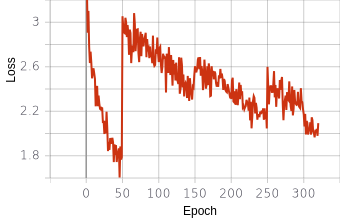
\includegraphics[width=\textwidth]{gambar/training_resnet50/tugas-akhir-Page 18.png}
		\caption*{(a) \textit{Training Loss}}
	\end{minipage}
	\hfill
	\begin{minipage}{0.45\textwidth}
		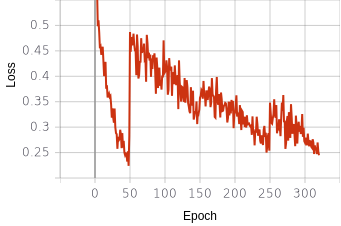
\includegraphics[width=\textwidth]{gambar/training_resnet50/tugas-akhir-Page 18 (1).png}
		\caption*{(b) \textit{Training Bounding Box Loss}}
	\end{minipage}
	\vfill
	\begin{minipage}{0.45\textwidth}
		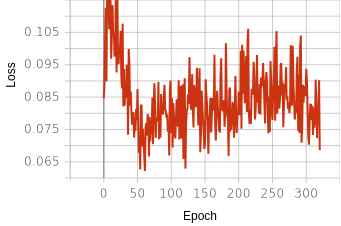
\includegraphics[width=\textwidth]{gambar/training_resnet50/tugas-akhir-Page 18 (2).png}
		\caption*{(c) \textit{Training Classification Loss}}
	\end{minipage}
	\hfill
	\begin{minipage}{0.45\textwidth}
		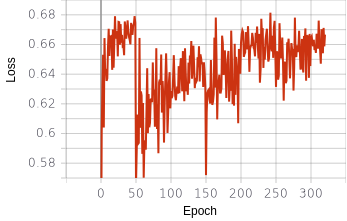
\includegraphics[width=\textwidth]{gambar/training_resnet50/tugas-akhir-Page 18 (3).png}
		\caption*{(d) \textit{Training Mask Loss}}
	\end{minipage}
	\caption{Grafik Perubahan \textit{Training Loss} pada \textit{MobileNet-V1}}
	\label{fig:mobilenetv1-training}
\end{figure}


Sedangkan pada saat proses \textit{validation} sendiri \textit{Loss} terendah yang berhasil dicapai pada \textit{epoch} ke 281 dengan nilai sebesar 1.624 dengan rincian \textit{validation bounding box loss} sebesar 0.2088, \textit{validation classification loss} sebesar 0.04799 serta \textit{validation mask loss} sebesar 0.6001. Namun untuk \textit{validation bounding box loss} terendah berada pada \textit{epoch} ke 300 dengan nilai sebesar 0.1927 sedangkan \textit{validation classification loss} terendah pada \textit{epoch} ke 70 dengan nilai 0.02607 serta \textit{validation mask loss} terendah pada \textit{epoch} ke 295 dengan nilai 0.5625. Gambar \ref{fig:mobilenetv1-val} merupakan grafik yang menunjukkan perubahan \textit{validation loss, validation bounding box loss, validation classification loss,} serta \textit{validation mask loss} dari \textit{epoch} 1 sampai 300.

\begin{figure}[H]
	\centering
	\begin{minipage}{0.45\textwidth}
		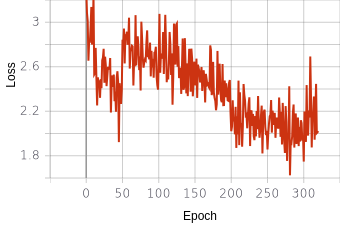
\includegraphics[width=\textwidth]{gambar/training_resnet50/tugas-akhir-Page 19.png}
		\caption*{(a) \textit{Validation Loss}}
	\end{minipage}
	\hfill
	\begin{minipage}{0.45\textwidth}
		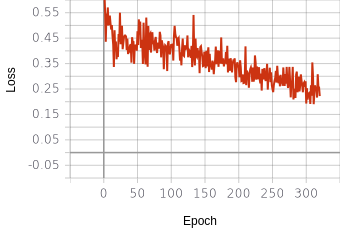
\includegraphics[width=\textwidth]{gambar/training_resnet50/tugas-akhir-Page 19 (1).png}
		\caption*{(b) \textit{Validation Bounding Box Loss}}
	\end{minipage}
	\vfill
	\begin{minipage}{0.45\textwidth}
		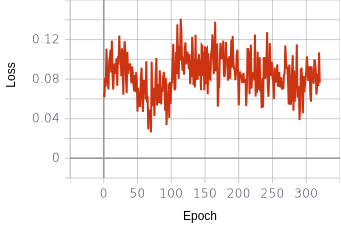
\includegraphics[width=\textwidth]{gambar/training_resnet50/tugas-akhir-Page 19 (2).png}
		\caption*{(c) \textit{Validation Classification Loss}}
	\end{minipage}
	\hfill
	\begin{minipage}{0.45\textwidth}
		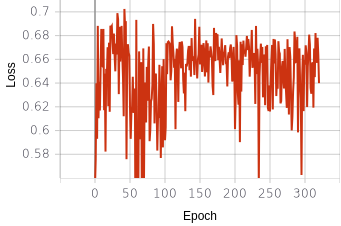
\includegraphics[width=\textwidth]{gambar/training_resnet50/tugas-akhir-Page 19 (3).png}
		\caption*{(d) \textit{Validation Mask Loss}}
	\end{minipage}
	\caption{Grafik Perubahan \textit{Validation Loss} pada \textit{MobileNet-V1}}
	\label{fig:mobilenetv1-val}
\end{figure}

Nilai \textit{mAP} tertinggi didapatkan pada \textit{epoch} ke 210 sebesar 26.04. Gambar \ref{fig:mobilenetv1-map} merupakan grafik yang menunjukan perubahan \textit{validation mean Average Precision} dari \textit{epoch} 1 sampai 300.


\begin{figure}[H]
	\centering
	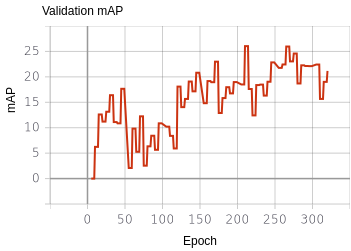
\includegraphics[scale=0.4]{gambar/mobilenetv1-map.png}
	\caption{Grafik Perubahan \textit{Validation mAP} pada \textit{MobileNet-V1}}
	\label{fig:mobilenetv1-map}
\end{figure} 

Tabel \ref{tab:train-recap} adalah tabel perbandingan dari \textit{output file size} dan \textit{mAP} dari total 3 model dengan \textit{backbone} berbeda yang diuji. Tahap ini masih merupakan hasil tahap \textit{training}. Sedangkan Gambar \ref{fig:graph-recap} merupakan grafik perbandingan \textit{mAP} dengan \textit{file size}. Proses selanjutnya setelah mendapatkan hasil yang ditunjukkan pada setiap model adalah melakukan proses prediksi atau melakukan \textit{testing data}.

\begin{table}[H]
	\centering
	\caption{Tabel Perbandingan Model dengan \textit{backbone} yang berbeda}
	\begin{tabular}{|c|l|l|l|}
		\hline
		\textbf{No.} & \multicolumn{1}{c|}{\textit{\textbf{Backbone}}} & \multicolumn{1}{c|}{\textit{\textbf{Output File Size}}} & \multicolumn{1}{c|}{\textbf{mAP}} \\ \hline
		1            & Resnet-50                                       & 170.9 MB                                                & 94.92\%                           \\ \hline
		2            & Resnet-101                                      & 244 MB                                                  & 96.21\%                           \\ \hline
		3            & Mobilenet-V1                                    & 83.3 MB                                                 & 26.04\%                           \\ \hline
	\end{tabular}
	\label{tab:train-recap}
\end{table}

\newpage

\begin{figure}[H]
	\centering
	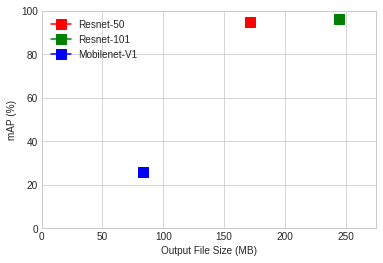
\includegraphics[scale=0.75]{gambar/graph-recap.png}
	\caption{Grafik Perbandingan Model dengan \textit{backbone} yang berbeda}
	\label{fig:graph-recap}
\end{figure}

\subsection{Perbandingan Hasil Prediksi}
\label{subsec:perbandingan-hasil-prediksi}

Setelah mendapatkan hasil \textit{training} pada Tabel \ref{tab:train-recap} terdapat dua parameter yang digunakan yaitu \textit{output file size} dan \textit{mean Average Precision}. Parameter tersebut digunakan untuk melakukan justifikasi dalam pemilihan model yang terbaik. Pada parameter \textit{output file size}, model yang diinginkan adalah model dengan dengan ukuran sekecil mungkin, agar tidak menghabiskan kapasitas penyimpanan terlalu banyak. Sedangkan untuk \textit{mean Average Precision} yang diinginkan adalah model dengan \textit{meand Average Precision} yang tinggi sehingga kemam puan model tersebut untuk melakukan proses prediksi akan semakin tepat dengan kondisi yang sesuai pada dunia nyata.

Setelah membandingkan parameter \textit{output file size} dan \textit{mean Average Precision}, pada tahap selanjutnya akan dilakukan proses membandingkan nilai atau hasil dari prediksi pada setiap model yang telah dibuat. Semakin tinggi \textit{mean Average Precision} dan kebenaran dalam prediksi, maka model tersebut sangat bagus dan sesuai dengan permasalahan yang ingin diselesaikan oleh model yang telah dibuat. Tujuan dari tahapan membandingkan ini adalah untuk memilih model yang terbaik dan apakah model yang telah dibuat dapat benar-benar dapat menyelesaikan permasalahan \textit{object detection and segmentation}. Sehingga, dari hasil percobaan ini dapat menentukan model terbaik yang dapat menyelesaikan permasalahan dan juga telah diuji dengan menggunakan\textit{ testing set}.

\subsubsection{Hasil Pengujian dengan \textit{Backbone Resnet-50}}

Pada hasil pengujian dengan menggunakan satu gambar jalan raya pada pada saat pagi hari yang ditunjukkan pada gambar \ref{fig:hasil-resnet50}, didapatkan hasil skor yaitu :
\begin{enumerate}[nolistsep]
	\item Pejalan kaki (\textit{score} : 0,984)
	\item \textit{Zebracross} (\textit{score} : 0,983)
\end{enumerate}
Dari hasil tersebut, \textit{Backbone Resnet-50} dapat memprediksi gambar dengan benar, serta \textit{evaluation time} dari \textit{backbone} ini sebesar 0,76 detik
\begin{figure}[H] 
	\centering
	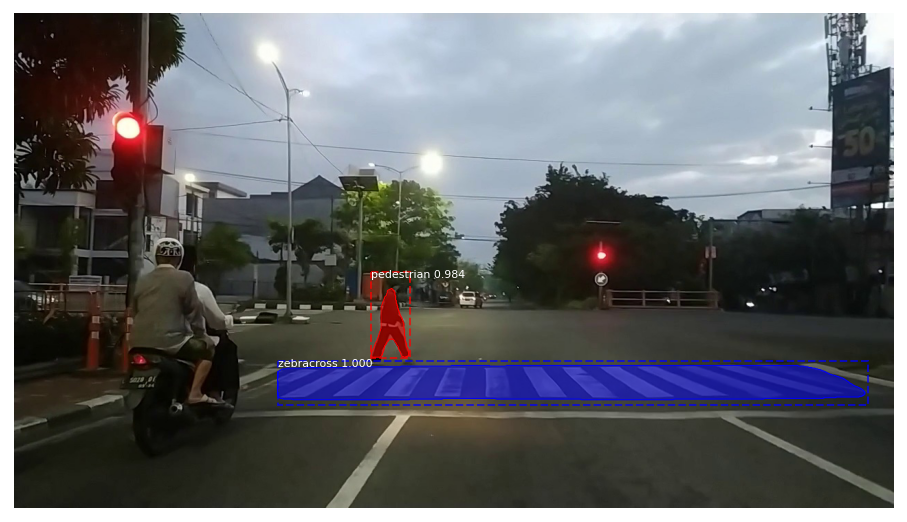
\includegraphics[scale=0.3]{gambar/hasil/resnet-50_fajar_800.png}
	\caption{Hasil Uji dari \textit{Backbone Resnet-50}}
	\label{fig:hasil-resnet50}
\end{figure}

\subsubsection{Hasil Pengujian dengan \textit{Backbone Resnet-101}}

Pada hasil pengujian dengan menggunakan satu gambar jalan raya pada pada saat pagi hari yang ditunjukkan pada gambar \ref{fig:hasil-resnet101}, didapatkan hasil skor yaitu :
\begin{enumerate}[nolistsep]
	\item Pejalan kaki (\textit{score} : 0,986)
	\item \textit{Zebracross} (\textit{score} : 0,995)
\end{enumerate}
Dari hasil tersebut, \textit{Backbone Resnet-101} dapat memprediksi gambar dengan benar, serta \textit{evaluation time} dari \textit{backbone} ini sebesar 0.961 detik
\begin{figure}[H] 
	\centering
	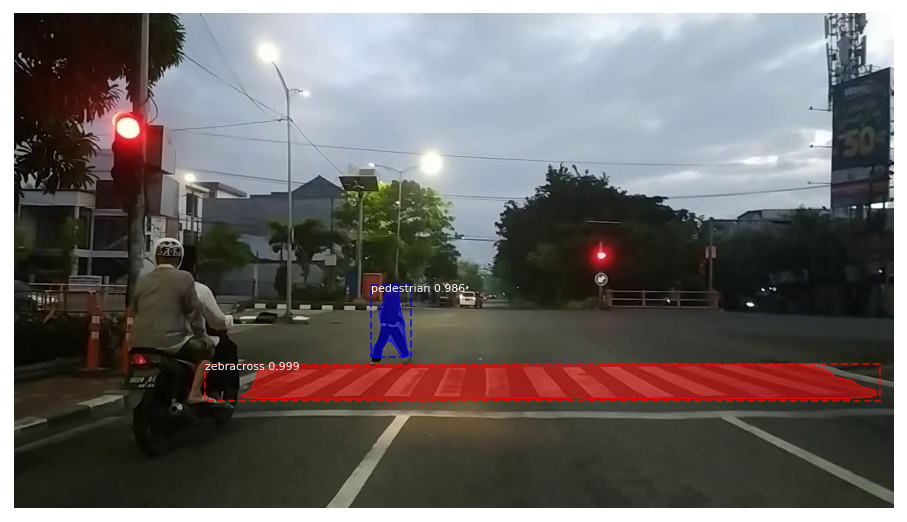
\includegraphics[scale=0.3]{gambar/hasil/resnet-101_fajar_800.png}
	\caption{Hasil Uji dari \textit{Backbone Resnet-101}}
	\label{fig:hasil-resnet101}
\end{figure}

\subsubsection{Hasil Pengujian dengan \textit{Backbone Mobilenet-V1}}

Pada hasil pengujian dengan menggunakan satu gambar jalan raya pada pada saat pagi hari yang ditunjukkan pada gambar \ref{fig:hasil-mobilenetv1}, didapatkan hasil skor yaitu :
\begin{enumerate}[nolistsep]
	\item Pejalan kaki (tidak terdeteksi)
	\item \textit{Zebracross} (terdeteksi 2  dengan \textit{score} : 0,942 dan 0.888)
\end{enumerate}
Dari hasil tersebut, \textit{Backbone Mobilenet-V1} tidak dapat memprediksi gambar dengan benar, serta \textit{evaluation time} dari \textit{backbone} ini sebesar 0.664 detik
\begin{figure}[H] 
	\centering
	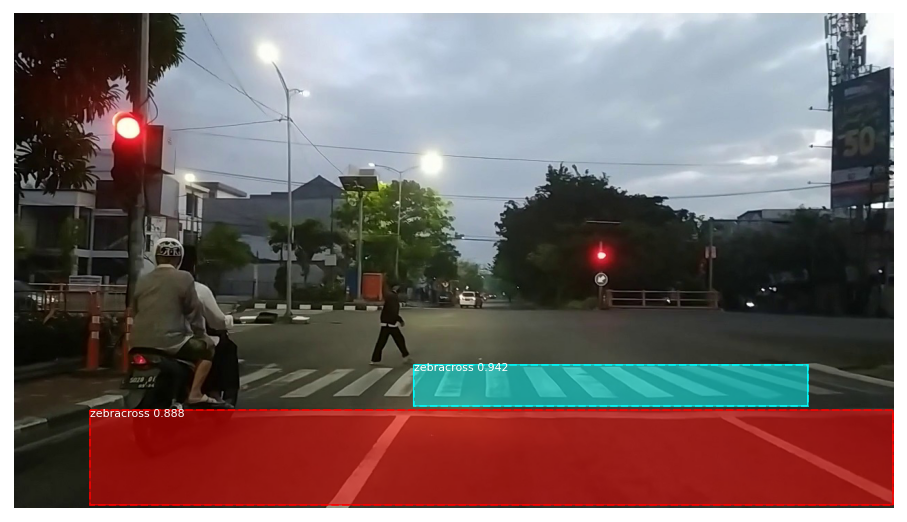
\includegraphics[scale=0.3]{gambar/fajar-frame800-mobilenetv1.png}
	\caption{Hasil Uji dari \textit{Backbone Mobilenet-V1}}
	\label{fig:hasil-mobilenetv1}
\end{figure}

Setelah melakukan \textit{testing} dengan menggunakan gambar pada \textit{testing set} pada keseluruhan model, maka tabel \ref{tab:result-comparasion} menunjukkan ringkasan dari perbandingan hasil \textit{testing} yang telah dilakukan. Parameter yang akan dibandingkan yaitu \textit{evaluation time} dan besar \textit{mean Average Precision}.

\begin{table}[H]
	\centering
	\caption{tabel Perbandingan Hasil \textit{Testing}}
	\resizebox{\textwidth}{!}{%
		\begin{tabular}{|c|l|r|r|}
			\hline
			\multicolumn{1}{|l|}{\textbf{No.}} & \textit{\textbf{Backbone}} & \textit{\textbf{Evaluation Time}} & \textbf{mAP} \\ \hline
			1                                  & ResNet-50                  & 0,763 s                           & 100\%        \\ \hline
			2                                  & ResNet-101                 & 0.961 s                             & 100\%        \\ \hline
			3                                  & MobileNet-v1               & 0.664 s                             & 25\%          \\ \hline
		\end{tabular}%
	}
	\label{tab:result-comparasion}
\end{table}

\section{Pengujian Perbedaan Waktu}
\label{sec:pengujian-waktu}

Pengujian pada perbedaan waktu bertujuan untuk mengetahui performa dan akurasi dari setiap model yang dihasilkan dengan waktu yang berbeda-beda (pagi, siang dan malam). \textit{File input} untuk pengujian ini terdapat 2 macam, yaitu gambar dengan format \textit{.jpg} dan video dengan format \textit{.mp4}.

\subsection{Pengujian di Pagi Hari}
\label{subsec:pagi}

Pada pengujian ini \textit{testing data} diambil dengan menggunakan kamera \textit{smartphone} yang menghasilkan video beresolusi 1280$\times$720 px berdurasi 63.43 s. Video tersebut mempunyai banyak \textit{frame} per detik sebanyak 30 fps serta total \textit{frame} yang dihasilkan sejumlah 1903 \textit{frame}. Gambar \ref{fig:comparasion-morning} merupakan perbandingan hasis deteksi dan segementasi dari ketiga \textit{backbone} yang digunakan pada waktu pagi hari.

\begin{figure}[H]
	\centering
	\begin{minipage}[b]{0.3\textwidth}
		\includegraphics[width=\textwidth]{gambar/hasil/resnet-50_fajar_800.png}
		\caption*{(a) ResNet-50}
	\end{minipage}
	\hfill
	\begin{minipage}[b]{0.3\textwidth}
		\includegraphics[width=\textwidth]{gambar/hasil/resnet-101_fajar_800.png}
		\caption*{(b) ResNet-101}
	\end{minipage}
	\hfill
	\begin{minipage}[b]{0.3\textwidth}
		\includegraphics[width=\textwidth]{gambar/fajar-frame800-mobilenetv1.png}
		\caption*{(c) MobileNet-v1}
	\end{minipage}
	\caption{{Perbandingan Hasil pada Pagi Hari}}
	\label{fig:comparasion-morning}
\end{figure}

Untuk meguji performa model yang dihasilkan pada masing-masing \textit{backbone}, digunakan beberapa parameter nilai seperti \textit{precision, recall} dan \textit{F1-score} pada masing-masing kelas objek yang dideteksi. Perbandingan hasil evaluasi yang didapatkan masing-masing \textit{backbone} dapat dilihat pada Tabel \ref{tab:evaluate-morning}.

Pada Resnet-50 \textit{Average Precision} untuk semua kelas yang berhasil dideteksi adalah sebesar 100\% dan \textit{Average Recall} 100\% dengan \textit{testing time} selama 0,763 s. Sedangkan pada Resnet-101 memberikan hasil yang sama dengan Resnet-50 dengan \textit{AP} 100\% dan \textit{AR} 100\% dengan \textit{testing time} selama 0,961 s. Namun pada Mobilenet-v1 objek yang berhasil dideteksi hanya \textit{zebracross} (ditambah dengan \textit{background}), sehingga pada objek pejalan kaki mempunyai \textit{Average Precision} bernilai 50\% serta \textit{Average Recall} dan \textit{F1-score} bernilai tidak terdefinisi atau \textit{NaN}. Hal ini dikarenakan nilai \textit{True Positif} pada pejalan kaki bernilai 0 (angka 0 dibagi nilai berapun memiliki hasil tidak terdefinisi) dengan \textit{testing time} selama 0.664 s.

\begin{table}[!h]
	\centering
	\caption{{Perbandingan Hasil Evaluasi pada Pagi Hari}}
	\begin{minipage}[b]{\textwidth}
		\centering
		\caption*{(a) ResNet-50}
		\begin{tabular}{|l|c|c|c|}
			\hline
			\multicolumn{1}{|c|}{\textbf{Kelas}} & \textit{\textbf{Precision (\%)}} & \textit{\textbf{Recall (\%)}} & \textit{\textbf{F1\_Score (\%)}} \\ \hline
			Background                           & 100                              & 100                           & 100                              \\ \hline
			Pedestrian                           & 100                              & 100                           & 100                              \\ \hline
			Zebracross                           & 100                              & 100                           & 100                              \\ \hline
		\end{tabular}
	\end{minipage}
	\vfill
	\begin{minipage}[b]{\textwidth}
		\centering
		\caption*{(b) ResNet-101}
		\begin{tabular}{|l|c|c|c|}
			\hline
			\multicolumn{1}{|c|}{\textbf{Kelas}} & \textit{\textbf{Precision (\%)}} & \textit{\textbf{Recall (\%)}} & \textit{\textbf{F1\_Score (\%)}} \\ \hline
			Background                           & 100                              & 100                           & 100                              \\ \hline
			Pedestrian                           & 100                              & 100                           & 100                              \\ \hline
			Zebracross                           & 100                              & 100                           & 100                              \\ \hline
			
		\end{tabular}
	\end{minipage}
	\vfill
	\begin{minipage}[b]{\textwidth}
		\centering
		\caption*{(c) MobileNet-v1}
		\begin{tabular}{|l|c|c|c|}
			\hline
			\multicolumn{1}{|c|}{\textbf{Kelas}} & \textit{\textbf{Precision (\%)}} & \textit{\textbf{Recall (\%)}} & \textit{\textbf{F1\_Score (\%)}} \\ \hline
			Background                           & 50                               & 50                         & 50                               \\ \hline
			Pedestrian                           & 0                                & NaN                           & NaN                              \\ \hline
			Zebracross                           & 100                              & 50                            & 66,67                            \\ \hline
			
		\end{tabular}
	\end{minipage}
	\label{tab:evaluate-morning}
\end{table}

Selain menggunakan \textit{input data} berupa gambar, pada pengujian ini juga menggunakan \textit{input data} berupa \textit{file} video dengan format \textit{.mp4}. Proses \textit{testing} dibagi menjadi dua tahapan, tahap pertama memecah \textit{frame} video menjadi gambar dan melakukan prediksi serta tahap kedua menggabungkan kembali setiap \textit{frame} menjadi video. Tabel \ref{tab:video_morning} menunjukan waktu yang dibutuhkan untuk melakukan semua tahap prediksi pada \textit{file input} berbentuk video pada ketiga \textit{backbone}.

\begin{table}[h]
	\centering{
		\caption{Waktu Prediksi pada \textit{File Input} Video dalam \textit{MM:SS}}
		\begin{tabular}{|l|c|c|c|c|}
			\hline
			\multicolumn{1}{|c|}{\textit{\textbf{Backbone}}} & \textit{\textbf{Tahap 1}} & \textit{\textbf{Tahap 2}} & \textit{\textbf{Total}} & \multicolumn{1}{l|}{\textit{\textbf{Output Size}}} 
			\\ \hline
			\textit{ResNet-50}                              & 07:24                     & 00:38                     & 08:03                   & 88.8 MB 
			\\ \hline
			\textit{ResNet-101}                                        & 07:54                     & 00:49                     & 08:44                   & 87.7 MB                                                                                       \\ \hline
			\textit{MobileNet-v1}                            & 06:50                     & 00:40                     & 07:31                   & 89.7 MB                                            \\ \hline
		\end{tabular}
	}
	\label{tab:video_morning}
\end{table}

\subsection{Pengujian di Siang Hari}
\label{subsec:siang}

Pada pengujian ini \textit{testing data} diambil dari video streaming \textit{youtube}\citep{test-siang} yang memiliki resolusi 1920$\times$1080 px berdurasi 29.4 s. Video tersebut mempunyai banyak \textit{frame} per detik sebanyak 25 fps serta total \textit{frame} yang dihasilkan sejumlah 735 \textit{frame}. Gambar \ref{fig:comparasion-afternoon} merupakan perbandingan hasis deteksi dan segementasi dari ketiga \textit{backbone} yang digunakan pada waktu siang hari.

\begin{figure}[!h]
	\centering
	\begin{minipage}[b]{0.3\textwidth}
		\includegraphics[width=\textwidth]{gambar/hasil/resnet-50_siang_465.png}
		\caption*{(a) ResNet-50}
	\end{minipage}
	\hfill
	\begin{minipage}[b]{0.3\textwidth}
		\includegraphics[width=\textwidth]{gambar/hasil/resnet-101_siang_465.png}
		\caption*{(b) ResNet-101}
	\end{minipage}
	\hfill
	\begin{minipage}[b]{0.3\textwidth}
		\includegraphics[width=\textwidth]{gambar/siang-frame465-mobilenetv1.png}
		\caption*{(c) MobileNet-v1}
	\end{minipage}
	\caption{{Perbandingan Hasil pada Siang Hari}}
	\label{fig:comparasion-afternoon}
\end{figure}

Perbandingan hasil evaluasi yang didapatkan masing-masing \textit{backbone} dengan membandingkan nilai \textit{precision, recall} dan \textit{F1-score} dapat dilihat pada Tabel \ref{tab:evaluate-afternoon}.

\begin{table}[!h]
	\centering
	\caption{{Perbandingan Hasil Evaluasi pada Siang Hari}}
	\begin{minipage}[b]{\textwidth}
		\centering
		\caption*{(a) ResNet-50}
		\begin{tabular}{|l|c|c|c|}
			\hline
			\multicolumn{1}{|c|}{\textbf{Kelas}} & \textit{\textbf{Precision (\%)}} & \textit{\textbf{Recall (\%)}} & \textit{\textbf{F1\_Score (\%)}} \\ \hline
			Background                           & 50                               & 100                            & 66,67                            \\ \hline
			Pedestrian                           & 100                              & 50                           & 66,67                              \\ \hline
			Zebracross                           & 100                               & 100                           & 100                            \\ \hline
			
		\end{tabular}
	\end{minipage}
	\vfill
	\begin{minipage}[b]{\textwidth}
		\centering
		\caption*{(b) ResNet-101}
		\begin{tabular}{|l|c|c|c|}
			\hline
			\multicolumn{1}{|c|}{\textbf{Kelas}} & \textit{\textbf{Precision (\%)}} & \textit{\textbf{Recall (\%)}} & \textit{\textbf{F1\_Score (\%)}} \\ \hline
			Background                           & 100                              & 100                            & 100                               \\ \hline
			Pedestrian                           & 100                              & 100                           & 100                              \\ \hline
			Zebracross                           & 100                               & 100                           & 100                            \\ \hline
			
		\end{tabular}
	\end{minipage}
	\vfill
	\begin{minipage}[b]{\textwidth}
		\centering
		\caption*{(c) MobileNet-v1}
		\begin{tabular}{|l|c|c|c|}
			\hline
			\multicolumn{1}{|c|}{\textbf{Kelas}} & \textit{\textbf{Precision (\%)}} & \textit{\textbf{Recall (\%)}} & \textit{\textbf{F1\_Score (\%)}} \\ \hline
			Background                           & 50                               & 66.67                         & 57,14                            \\ \hline
			Pedestrian                           & 0                                & NaN                           & NaN                              \\ \hline
			Zebracross                           & 100                               & 33,33                            & 50                               \\ \hline
			
		\end{tabular}
	\end{minipage}
	\label{tab:evaluate-afternoon}
\end{table}

Pada Resnet-50 \textit{Average Precision} untuk semua kelas yang berhasil dideteksi adalah sebesar 83.334\% dan \textit{Average Recall} 83.334\% dengan \textit{testing time} selama 1,253 s. Sedangkan pada Resnet-101 memberikan hasil \textit{AP} sebesar 100\% dan \textit{AR} 100\% dengan \textit{testing time} selama 1,549 s. Namun pada Mobilenet-v1 objek yang berhasil dideteksi hanya \textit{zebra cross} (ditambah dengan \textit{background}) sama saat pengujian pada pagi hari. Nilai \textit{AP} yang dihasilkan pada evaluasi Mobilenet-v1 sebesar 50\% dengan \textit{testing time} selama 1,186 s.

Selain menggunakan \textit{input data} berupa gambar, pada pengujian ini juga menggunakan \textit{input data} berupa \textit{file} video dengan format \textit{.mp4}. Proses \textit{testing} dibagi menjadi dua tahapan, tahap pertama memecah \textit{frame} video menjadi gambar dan melakukan prediksi serta tahap kedua menggabungkan kembali setiap \textit{frame} menjadi video. Tabel \ref{tab:video-afternoon} menunjukan waktu total yang dibutuhkan untuk melakukan semua tahap prediksi pada \textit{file input} berbentuk video pada ketiga \textit{backbone}.

\begin{table}[!h]
	\centering{
		\caption{Waktu Prediksi pada \textit{File Input} Video dalam \textit{MM:SS}}
		\begin{tabular}{|l|c|c|c|c|}
			\hline
			\multicolumn{1}{|c|}{\textit{\textbf{Backbone}}} & \textit{\textbf{Tahap 1}} & \textit{\textbf{Tahap 2}} & \textit{\textbf{Total}} & \multicolumn{1}{l|}{\textit{\textbf{Output Size}}} \\ \hline
			\textit{ResNet-50}                              & 05:33                     & 00:30                     & 06:03                    & 52.8 MB                                            \\ \hline
			\textit{ResNet-101}                                        & 07:21                     & 00:36                     & 07:58                   & 50.1 MB                                           \\ \hline
			\textit{MobileNet-v1}                            & 04:03                     & 00:30                     & 04:33                   & 42 MB                                              \\ \hline
		\end{tabular}
	}
	\label{tab:video-afternoon}
\end{table}

\subsection{Pengujian di Malam Hari}
\label{subsec:malam}

Pada pengujian ini \textit{testing data} diambil dari video \textit{streaming youtube} \citep{test-malam} yang memiliki resolusi 1920$\times$1080 px berdurasi 28.04 s. Video tersebut mempunyai banyak \textit{frame} per detik sebanyak 25 fps serta total \textit{frame} yang dihasilkan sejumlah 701 \textit{frame}. Gambar \ref{fig:comparasion-night} merupakan perbandingan hasis deteksi dan segementasi dari ketiga \textit{backbone} yang digunakan pada waktu siang hari.

\begin{figure}[H]
	\centering
	\begin{minipage}[b]{0.3\textwidth}
		\includegraphics[width=\textwidth]{gambar/hasil/resnet-50_malam_180.png}
		\caption*{(a) ResNet-50}
	\end{minipage}
	\hfill
	\begin{minipage}[b]{0.3\textwidth}
		\includegraphics[width=\textwidth]{gambar/hasil/resnet-101_malam_180.png}
		\caption*{(b) ResNet-101}
	\end{minipage}
	\hfill
	\begin{minipage}[b]{0.3\textwidth}
		\includegraphics[width=\textwidth]{gambar/malam-frame180-mobilnetv1.png}
		\caption*{(c) MobileNet-v1}
	\end{minipage}
	\caption{{Perbandingan Hasil pada Malam Hari}}
	\label{fig:comparasion-night}
\end{figure}

Perbandingan hasil evaluasi yang didapatkan masing-masing \textit{backbone} dengan membandingkan nilai \textit{precision, recall} dan \textit{F1-score} dapat dilihat pada Tabel \ref{tab:evaluate-night}.

\begin{table}[H]
	\centering
	\caption{{Perbandingan Hasil Evaluasi pada Malam Hari}}
	\begin{minipage}[b]{\textwidth}
		\centering
		\caption*{(a) ResNet-50}
		\begin{tabular}{|l|c|c|c|}
			\hline
			\multicolumn{1}{|c|}{\textbf{Kelas}} & \textit{\textbf{Precision (\%)}} & \textit{\textbf{Recall (\%)}} & \textit{\textbf{F1\_Score (\%)}} \\ \hline
			Background                           & 100                              & 25                            & 40                               \\ \hline
			Pedestrian                           & 40                               & 100                           & 57.14                            \\ \hline
			Zebracross                           & 100                              & 100                           & 100                              \\ \hline
			
		\end{tabular}	
		
	\end{minipage}
	\vfill
	\begin{minipage}[b]{\textwidth}
		\centering
		\caption*{(b) ResNet-101}
		\begin{tabular}{|l|c|c|c|}
			\hline
			\multicolumn{1}{|c|}{\textbf{Kelas}} & \textit{\textbf{Precision (\%)}} & \textit{\textbf{Recall (\%)}} & \textit{\textbf{F1\_Score (\%)}} \\ \hline
			Background                           & 100                              & 33.33                         & 50                               \\ \hline
			Pedestrian                           & 60                               & 100                           & 74.9                             \\ \hline
			Zebracross                           & 100                              & 100                           & 100                              \\ \hline
			
		\end{tabular}
		
	\end{minipage}
	\vfill
	\begin{minipage}[b]{\textwidth}
		\centering
		\caption*{(c) MobileNet-v1}
		\begin{tabular}{|l|c|c|c|}
			\hline
			\multicolumn{1}{|c|}{\textbf{Kelas}} & \textit{\textbf{Precision (\%)}} & \textit{\textbf{Recall (\%)}} & \textit{\textbf{F1\_Score (\%)}} \\ \hline
			Background                           & 50                               & 16,64                         & 28,57                               \\ \hline
			Pedestrian                           & 0                                & NaN                           & NaN                              \\ \hline
			Zebracross                           & 100                              & 100                            & 100                            \\ \hline
			
		\end{tabular}
		
	\end{minipage}
	
	\label{tab:evaluate-night}
\end{table}

Pada gambar yang diuji untuk malam hari hanya memiliki 2 kelas saja yaitu \textit{background}, pejalan kaki serta \textit{zebracross}. Resnet-50 mempunyai nilai \textit{Average Precision} untuk semua kelas yang berhasil dideteksi adalah sebesar 80\% dan \textit{Average Recall} 75\% dengan \textit{testing time} selama 1,069 s. Sedangkan pada Resnet-101 memberikan hasil \textit{AP} sebesar 86.67\% dan \textit{AR} 77.77\% dengan \textit{testing time} selama 1,215 s. Namun pada Mobilenet-v1 objek yang berhasil dideteksi hanya \textit{zebracross} (ditambah dengan \textit{background}) sama saat pengujian pada pagi dan siang hari. Nilai \textit{AP} yang dihasilkan pada evaluasi Mobilenet-v1 sebesar 66,67\% dengan \textit{testing time} selama 1,051 s.

Selain menggunakan \textit{input data} berupa gambar, pada pengujian ini juga menggunakan \textit{input data} berupa \textit{file} video dengan format \textit{.mp4}. Proses \textit{testing} dibagi menjadi dua tahapan, tahap pertama memecah \textit{frame} video menjadi gambar dan melakukan prediksi serta tahap kedua menggabungkan kembali setiap \textit{frame} menjadi video. Tabel \ref{tab:video-night} menunjukan waktu yang dibutuhkan untuk melakukan semua tahap prediksi pada \textit{file input} berbentuk video pada ketiga \textit{backbone}.

\begin{table}[H]
	\centering{
		\caption{Waktu Prediksi pada \textit{File Input} Video dalam \textit{MM:SS}}
		\begin{tabular}{|l|c|c|c|l|}
			\hline
			\multicolumn{1}{|c|}{\textit{\textbf{Backbone}}} & \textit{\textbf{Tahap 1}} & \textit{\textbf{Tahap 2}} & \textit{\textbf{Total}} & \textit{\textbf{Output Size}} \\ \hline
			\textit{ResNet-50}                              & 04:23                     & 00:28                     & 04:51                     & 38.7 MB                     \\ \hline
			\textit{ResNet-101}                                        & 04:49                     & 00:34                     & 05:23                   & 39.1 MB                       \\ \hline
			\textit{MobileNet-v1}                            & 03:39                     & 00:28                     & 04:07                   & 36.1 MB                       \\ \hline
		\end{tabular}
	}
	\label{tab:video-night}
\end{table}


\subsection{Perbandingan Hasil Evaluasi pada Perbedaan Waktu}
\label{subsec:compare-eval}

Setelah membandingkan hasil evaluasi model setiap perbedaan waktu, pada bagian ini akan dibandingkan peforma setiap model untuk keseluruhan perbedaan waktu (pagi, siang dan malam hari). 

\subsubsection{ResNet-50}

Pada proses evaluasi model dengan menggunakan seluruh \textit{testing data} (pagi, siang dan malam hari) didapatkan beberapa hasil skor yaitu :
\begin{enumerate}[nolistsep]
	\item \textit{mean Average Precision(mAP)} : 77.381\%
	\item \textit{mean Average Recall(mAR)} : 76.667\%
	\item \textit{F1-score} : 75.555\%
\end{enumerate}
Hasil tersebut didapatkan setelah dilakukan proses pencarian nilai \textit{Trur Positif, False Positif} dan \textit{False Negatif} seperti yang ditunjukkan pada \textit{confusion matrix} pada Gambar \ref{fig:confmatrix-resnet50}.

\begin{figure}[H]
	\centering
	\includegraphics[scale=0.3]{gambar/confmatrix/resnet50_confmat.png}
	\caption{\textit{Confusion Matrix} ResNet-50}
	\label{fig:confmatrix-resnet50}
\end{figure}

\subsubsection{ResNet-101}

Pada proses evaluasi model dengan menggunakan seluruh \textit{testing data} (pagi, siang dan malam hari) didapatkan beberapa hasil skor yaitu :
\begin{enumerate}[nolistsep]
	\item \textit{mean Average Precision(mAP)} : 90.476\%
	\item \textit{mean Average Recall(mAR)} : 88.889\%
	\item \textit{F1-score} : 87.777\%
\end{enumerate}
Hasil tersebut didapatkan setelah dilakukan proses pencarian nilai \textit{Trur Positif, False Positif} dan \textit{False Negatif} seperti yang ditunjukkan pada \textit{confusion matrix} pada Gambar \ref{fig:confmatrix-resnet101}.

\begin{figure}[H]
	\centering
	\includegraphics[scale=0.3]{gambar/confmatrix/resnet-101_confmat.png}
	\caption{\textit{Confusion Matrix} ResNet-101}
	\label{fig:confmatrix-resnet101}
\end{figure}

\subsubsection{MobileNet-v1}

Pada proses evaluasi model dengan menggunakan seluruh \textit{testing data} (pagi, siang dan malam hari) didapatkan beberapa hasil skor yaitu :
\begin{enumerate}[nolistsep]
	\item \textit{mean Average Precision(mAP)} : 52.381\%
	\item \textit{mean Average Recall(mAR)} : \textit{NaN}
	\item \textit{F1-score} : \textit{NaN}
\end{enumerate}
Hasil tersebut didapatkan setelah dilakukan proses pencarian nilai \textit{Trur Positif, False Positif} dan \textit{False Negatif} seperti yang ditunjukkan pada \textit{confusion matrix} pada Gambar \ref{fig:confmatrix-mobilenetv1}.

\begin{figure}[H]
	\centering
	\includegraphics[scale=0.3]{gambar/confmatrix/mobilenetv1_confmat.png}
	\caption{\textit{Confusion Matrix} MobileNet-v1}
	\label{fig:confmatrix-mobilenetv1}
\end{figure}
  \cleardoublepage

  % Bab 5 penutup
  \chapter{PENUTUP}
\label{chap:penutup}

% Ubah bagian-bagian berikut dengan isi dari penutup

\section{Kesimpulan}
\label{sec:kesimpulan}

Berdasarkan hasil pengujian yang telah dilakukan, penulis dapat menyimpulkan beberapa hal sebagai berikut:

\begin{enumerate}[nolistsep]

  \item Dalam penelitian ini telah diimplementasikan dengan baik proses pendeteksian pejalan kaki dan zebracross dengan menggunakan Mask R-CNN, dengan \textit{mean Average Precision} sebesar 76.62\%.
  \item \textit{Backbone} ResNet-101 memiliki hasil akurasi yang lebih baik dibanding dengan \textit{backbone} lainnya dengan peforma lebih tinggi sebesar 12.82\% dibanding ResNet-50 dan 67.36\% dibanding MobileNet-v1. 
  \item Waktu yang dibutuhkan dalam proses pendektesian akan semakin lama jika objek yang berada pada gambar semakin banyak.
  
\end{enumerate}

\section{Saran}
\label{sec:saran}

Untuk pengembangan lebih lanjut pada penelitian mendatang, maka penulis memiliki saran sebagai berikut:

\begin{enumerate}[nolistsep]

  \item Menambah jumlah sample data pada kelas pengendara motor yang dinilai masih sedikit untuk dataset yang dipilih.

  \item Pembuatan dataset pejalan kaki di Indonesia karena perilaku pejalan kaki antar negara memiliki perbedaan yang cukup signifikan.

\end{enumerate}

  \cleardoublepage

  % Daftar pustaka
  \renewcommand\bibname{DAFTAR PUSTAKA}
  \addcontentsline{toc}{chapter}{\bibname}
  \bibliographystyle{unsrtnat}
  \bibliography{pustaka/pustaka.bib}
  \cleardoublepage

  % Biografi penulis
  \begin{center}
  \Large
  \textbf{BIOGRAFI PENULIS}
\end{center}

\addcontentsline{toc}{chapter}{BIOGRAFI PENULIS}

\vspace{2ex}

\begin{wrapfigure}{L}{0.3\textwidth}
  \centering
  \vspace{-3ex}
  % Ubah file gambar berikut dengan file foto dari mahasiswa
  \includegraphics[width=0.3\textwidth]{gambar/agung.jpg}
  \vspace{-4ex}
\end{wrapfigure}

% Ubah kalimat berikut dengan biografi dari mahasiswa
Agung Wicaksono, atau biasa dipanggil Agung, lahir di Madiun Jawa Timur pada tanggal 20 Mei 1999. Merupakan anak kedua dari tiga bersaudara. Penulis lulus dari SMP Negeri 1 Geger dan melanjutkan ke SMA Negeri 1 Geger. Penulis melanjutkan ke jenjang strata satu di Departemen Teknik Komputer Fakultas Teknologi Elektro dan Informatika Cerdas ITS. Dalam masa perkuliahan, penulis tertarik dengan pengembangan \textit{Web Apps} dan \textit{Machine Learning}. Penulis pernah aktif menjadi Staf Departemen Pengembangan Sumber Daya Mahasiswa Badan Eksekutif Mahasiswa Fakultas Teknologi Elektro serta Staf Ahli Kestari Mage 5. Bagi pembaca yang mamiliki kritik, saran, atau pertanyaan mengenai tugas akhir ini dapat menghubungi penulis melalui email wicaksonoagun05@gmail.com.

  \cleardoublepage

\end{document}
